\documentclass[handout]{beamer}

%\documentclass[compress]{beamer}

%\documentclass{beamer}
\usepackage[T1]{fontenc}
\usepackage{pifont}
\usepackage{threeparttable}
\usepackage{subcaption}
\usepackage{tikz-qtree}
\usepackage{listings}
\usepackage[american]{babel}
\usepackage{csquotes}
\usepackage[style=apa, backend=biber]{biblatex}
\usepackage{tikz}
\usepackage{multicol}
\usepackage{booktabs}
\usepackage{graphicx}
\usepackage{neuralnetwork}
\usepackage{hyperref}

\usepackage{minted}
\definecolor{listingbg}{rgb}{0.87,0.93,1}
\setminted[python]{
breaklines,
linenos,
fontsize=\scriptsize,
frame=single,
xleftmargin=0pt}

\hypersetup{
    pdfborder={0 0 0},
    colorlinks=true,
}
\usetheme[block=fill,subsectionpage=progressbar,sectionpage=progressbar]{metropolis} 

\definecolor{Purple}{HTML}{911146}
\definecolor{Orange}{HTML}{CF4A30}

\setbeamercolor{alerted text}{fg=Orange}
\setbeamercolor{frametitle}{bg=Purple}

\setbeamercovered{still covered={\opaqueness<1->{5}},again covered={\opaqueness<1->{100}}}

\lstset{
    basicstyle=\scriptsize\ttfamily,
    columns=flexible,
    breaklines=true,
    numbers=left,
    %stepsize=1,
    numberstyle=\tiny,
    backgroundcolor=\color[rgb]{0.85,0.90,1}
}

\lstnewenvironment{lstlistingoutput}{\lstset{
        basicstyle=\footnotesize\ttfamily,
        columns=flexible,
        breaklines=true,
        numbers=left,
        %stepsize=1,
        numberstyle=\tiny,
        backgroundcolor=\color[rgb]{.7,.7,.7}}}{}


\lstnewenvironment{lstlistingoutputtiny}{\lstset{
        basicstyle=\tiny\ttfamily,
        columns=flexible,
        breaklines=true,
        numbers=left,
        %stepsize=1,
        numberstyle=\tiny,
        backgroundcolor=\color[rgb]{.7,.7,.7}}}{}

\renewcommand*{\bibfont}{\tiny}

\makeatletter
\setbeamertemplate{headline}{%
    \begin{beamercolorbox}[colsep=1.5pt]{upper separation line head}
    \end{beamercolorbox}
    \begin{beamercolorbox}{section in head/foot}
        \vskip2pt\insertnavigation{\paperwidth}\vskip2pt
    \end{beamercolorbox}%
    \begin{beamercolorbox}[colsep=1.5pt]{lower separation line head}
    \end{beamercolorbox}
}
\makeatother

\newcommand{\question}[1]{
    \begin{frame}[plain]
        \begin{columns}
            \column{.4\textwidth}
            \makebox[\columnwidth]{
                
\includegraphics[width=\columnwidth,height=\paperheight,keepaspectratio]{mannetje.png}}
            \column{.6\textwidth}
            \large
            \textcolor{orange}{\textbf{\emph{#1}}}
        \end{columns}
    \end{frame}}

\newcommand{\instruction}[1]{\emph{\textcolor{gray}{[#1]}}}

\addbibresource{../resources/literature.bib}
\graphicspath{{../resources/pictures/}}

\title[Computational Communication Science 2]{\textbf{Computational Communication Science 2} \\Week 3 - Lecture\\ »LDA and Recommender systems«}
\author[Anne Kroon]{Anne Kroon \\ ~ \\ \footnotesize{ a.c.kroon@uva.nl, @annekroon} \\}
\date{April 15, 2024}
\institute[Digital Society Minor, University of Amsterdam]{Digital Society Minor, University of Amsterdam}

\begin{document}
	
	\begin{frame}{}
		\titlepage
	\end{frame}
	
	\begin{frame}{Today}
		\begin{tiny}
		\tableofcontents
		\end{tiny}
	\end{frame}

\question{Everything clear from last weeks?}


	\begin{frame}{Main points from last week}
		\begin{alertblock}{I assume that by now, everybody knows:}
			\begin{itemize}[<+>]
				\item how to clean and preprocess textual data;
				\item how to vectorize the data;
				\item how to calculate cosine similarity using different techniques;
			\end{itemize}
		\end{alertblock}
	\end{frame}

\section{Topic modelling}

\begin{frame}{Let's assume you want to know a bit more about the \emph{content} you are investigating}
Cosine and soft cosine do \emph{not} inform us about substantive issues present in text. 
	\begin{enumerate}
		\item Which topics can we extract from the corpus?
		\item How present is each of these topics in each text in the corpus?
	\end{enumerate}
\end{frame}

\begin{frame}[fragile]{Recap: Document-term matrix}
	Document-term matrix
	\begin{lstlisting}
      w1,w2,w3,w4,w5,w6 ...
text1, 2, 0, 0, 1, 2, 3 ...
text2, 0, 0, 1, 2, 3, 4 ...
text3, 9, 0, 1, 1, 0, 0 ...
...
	\end{lstlisting}
	{\small{These can be simple counts, but also more advanced metrics, like tf-idf scores (where you weigh the frequency by the number of documents in which it occurs), cosine distances, etc.}}
	\pause
	\begin{itemize}
		\item given a term-document matrix, easy to do with any tool
		\item probably extremely skewed distributions
	\end{itemize}
	
\end{frame}


\begin{frame}{Recap: clustering}
	\begin{itemize}
		\item given a term-document matrix, we can easily find clusters of documents that resemble each other
	\end{itemize}
\end{frame}


\begin{frame}{We need other models to}
	\begin{enumerate}[<+->]
		\item model \emph{simultaneously} (a) which topics we find in the whole corpus, and (b) which of these topics are present in which document; while at the same time
		\item allowing (a) words to be part of multiple topics, and (b) multiple topics to be present in one document; and
		\item being able to make connections between words ``even if they never actually occured in a document together'' \parencite{Maier2018}[p.~96]
	\end{enumerate}
	
	\tiny{Maier, D., Waldherr, A., Miltner, P., Wiedemann, G., Niekler, A., Keinert, A., \ldots Adam, S. (2018). Applying LDA Topic Modeling in Communication Research: Toward a Valid and Reliable Methodology. \textit{Communication Methods and Measures, 12}(2--3), 93--118. doi:10.1080/19312458.2018.1430754}
\end{frame}


\subsection{An introduction to LDA}

\begin{frame}{}
	Enter \textbf{topic modeling with Latent Dirichlet Allocation (LDA)}
\end{frame}


\begin{frame}{LDA, what's that?}
	\begin{block}{No mathematical details here, but the general idea}
		\begin{itemize}
			\item There are $k$ topics, $T_1$\ldots$T_k$
			\item Each document $D_i$ consists of a mixture of these topics, e.g.$80\% T_1, 15\% T_2, 0\% T_3, \ldots 5\% T_k $
			\item On the next level, each topic consists of a specific probability distribution of words
			\item Thus, based on the frequencies of words in $D_i$, one can infer its distribution of topics
			\item Note that LDA is a Bag-of-Words (BOW) approach
		\end{itemize}
	\end{block}
	
\end{frame}


\begin{frame}[fragile]{Doing a LDA in Python}
We will use gensim \parencite{Rehurek10softwareframework} for this (make sure you have version >4.0)
	
Let us assume you have a list of lists of documents called \texttt{texts}:
\begin{minted}[%
	breaklines,
	linenos,
	fontsize=\tiny,
	frame=single,
	xleftmargin=0pt,]
	{python}
print(texts[0][:115])
\end{minted}
\pause
which looks something like:
\begin{minted}[%
	fontsize=\tiny,
	breaklines,]
	{python}
'Stop the presses: CNN covered some actual news yesterday when it reported on the story of medical kidnapping victim Alyssa Gilderhus at the Mayo Clinic. But was it actually InfoWars and FreeMartyG which publicly shamed CNN into doing this real journalism? Cue the Mission Impossible theme music for this one...\n\nThis mission, as we accepted it, began more than a year ago during the baby Charlie Gard medical kidnapping scandal in the UK and we thought that it had ended with an apparently unsuccessf'
\end{minted}
	
	\tiny{{\v R}eh{\r u}{\v r}ek, R., \& Sojka, P. (2010). Software framework for topic modelling with large corpora. \emph{Proceedings of the LREC 2010 Workshop on New Challenges for NLP Frameworks}, pp. 45–50. Valletta, Malta: ELRA. }
\end{frame}

\begin{frame}[fragile]{Preprocessing}
Your preprocessing steps and feature engineering decisions \emph{largely} affect your topics
	\begin{enumerate}
		\item<1-> You can apply 'manual' preprocessing steps \dots
		\item<2->\dots In isolation or combination with for example \texttt{tfidf} transformations
	\end{enumerate}
\pause
\pause
\begin{minted}[%
breaklines,
linenos,
fontsize=\tiny,
frame=single,
xleftmargin=0pt,]
{python}
texts_clean = [text.lower() for text in texts]
texts_clean=[" ".join(text.split()) for text in texts_clean]  #remove dubble spaces
texts_clean = ["".join([l for l in text if l not in punctuation]) for text in texts_clean] #remove punctuaction
texts_clean[0][:500]
\end{minted}
\pause
which looks something like:
\begin{minted}[%
breaklines,
fontsize=\tiny,]
{python}
'stop the presses cnn covered some actual news yesterday when it reported on the story of medical kidnapping victim alyssa gilderhus at the mayo clinic but was it actually infowars and freemartyg which publicly shamed cnn into doing this real journalism cue the mission impossible theme music for this one this mission as we accepted it began more than a year ago during the baby charlie gard medical kidnapping scandal in the uk and we thought that it had ended with an apparently unsuccessful april '
\end{minted}
\end{frame}


\begin{frame}[fragile]{Preprocessing}
Without \emph{stopword removal},  \emph{tfidf} transformation and/or \emph{pruning}, you topics will not be very informative.
\pause
	\begin{minted}[%
		breaklines,
		linenos,
		fontsize=\tiny,
		frame=single,
		xleftmargin=0pt,]
		{python}
mystopwords = set(stopwords.words('english')) # use default NLTK stopword list; alternatively:
# mystopwords = set(open('mystopwordfile.txt').readlines())  #read stopword list from a textfile with one stopword per line
texts_clean = [" ".join(word for word in text.split() if word not in mystopwords) for text in texts_clean]
texts_clean[0][:500]
	\end{minted}
	\pause
	which looks something like:
	\begin{minted}[%
		breaklines,
		fontsize=\tiny,]
		{python}
'stop presses cnn covered actual news yesterday reported story medical kidnapping victim alyssa gilderhus mayo clinic actually infowars freemartyg publicly shamed cnn real journalism cue mission impossible theme music one mission accepted began year ago baby charlie gard medical kidnapping scandal uk thought ended apparently unsuccessful april fools joke cnn sure many recall charlie gard infant rare form otherwise notsorare condition mitochondrial disease story went viral made international news '
	\end{minted}
\end{frame}

\begin{frame}[fragile]{Tokenization}
\texttt{gensim} expects a list of words (hence: \texttt{tokenize} your corpus)
	\pause
\begin{minted}[%
		breaklines,
		linenos,
		fontsize=\tiny,
		frame=single,
		xleftmargin=0pt,]
		{python}
tokenized_texts_clean = [TreebankWordTokenizer().tokenize(text) for text in texts_clean ] # tokenize texts; convert all strings to a list of tokens
tokenized_texts_clean[0][:500]
	\end{minted}
	\pause
	which looks something like:
	\begin{minted}[%
		breaklines,
		fontsize=\tiny,]
		{python}
['stop',
'presses',
'cnn',
'covered',
'actual',
'news',
'yesterday',
'reported',
'story',
..
	\end{minted}
\end{frame}

\begin{frame}[fragile]{LDA implementation}
	\texttt{LDA} implementation
	\pause
	\begin{minted}[%
		breaklines,
		linenos,
		fontsize=\tiny,
		frame=single,
		xleftmargin=0pt,]
		{python}
raw_m1 = tokenized_texts_clean

# assign a token_id to each word
id2word_m1 = corpora.Dictionary(raw_m1)   
# represent each text by (token_id, token_count) tuples
ldacorpus_m1 = [id2word_m1.doc2bow(text) for text in raw_m1] 

#estimate the model
lda_m1 = models.LdaModel(ldacorpus_m1, id2word=id2word_m1, num_topics=10)
lda_m1.print_topics()
	\end{minted}
	\pause

\begin{minted}[%
		breaklines,
		fontsize=\tiny,]
		{python}
[(0,
'0.015*"trump" + 0.012*"said" + 0.006*"president" + 0.006*"people" + 0.004*"cnn" + 0.004*"us" + 0.004*"house" + 0.004*"news" + 0.003*"also" + 0.003*"twitter"'),
(1,
'0.010*"said" + 0.008*"trump" + 0.004*"one" + 0.004*"people" + 0.004*"us" + 0.004*"president" + 0.004*"would" + 0.003*"media" + 0.003*"also" + 0.003*"new"'),
(2,
'0.011*"trump" + 0.009*"said" + 0.007*"president" + 0.005*"would" + 0.004*"people" + 0.004*"us" + 0.003*"also" + 0.003*"like" + 0.003*"news" + 0.003*"state"'),
(3,
'0.010*"trump" + 0.006*"president" + 0.005*"said" + 0.004*"would" + 0.004*"us" + 0.003*"also" + 0.003*"people" + 0.003*"media" + 0.003*"news" + 0.003*"one"'),
\end{minted}
\end{frame}




\begin{frame}[fragile]{Visualization with pyldavis}
	\begin{minted}[%
	breaklines,
	linenos,
	fontsize=\tiny,
	frame=single,
	xleftmargin=0pt,]
	{python}
import pyLDAvis
import pyLDAvis.gensim_models as gensimvis
# first estiate gensim model, then:
vis_data = gensimvis.prepare(lda_m1,ldacorpus_m1,id2word_m1)
pyLDAvis.display(vis_data)
\end{minted}
	\makebox[\linewidth]{
		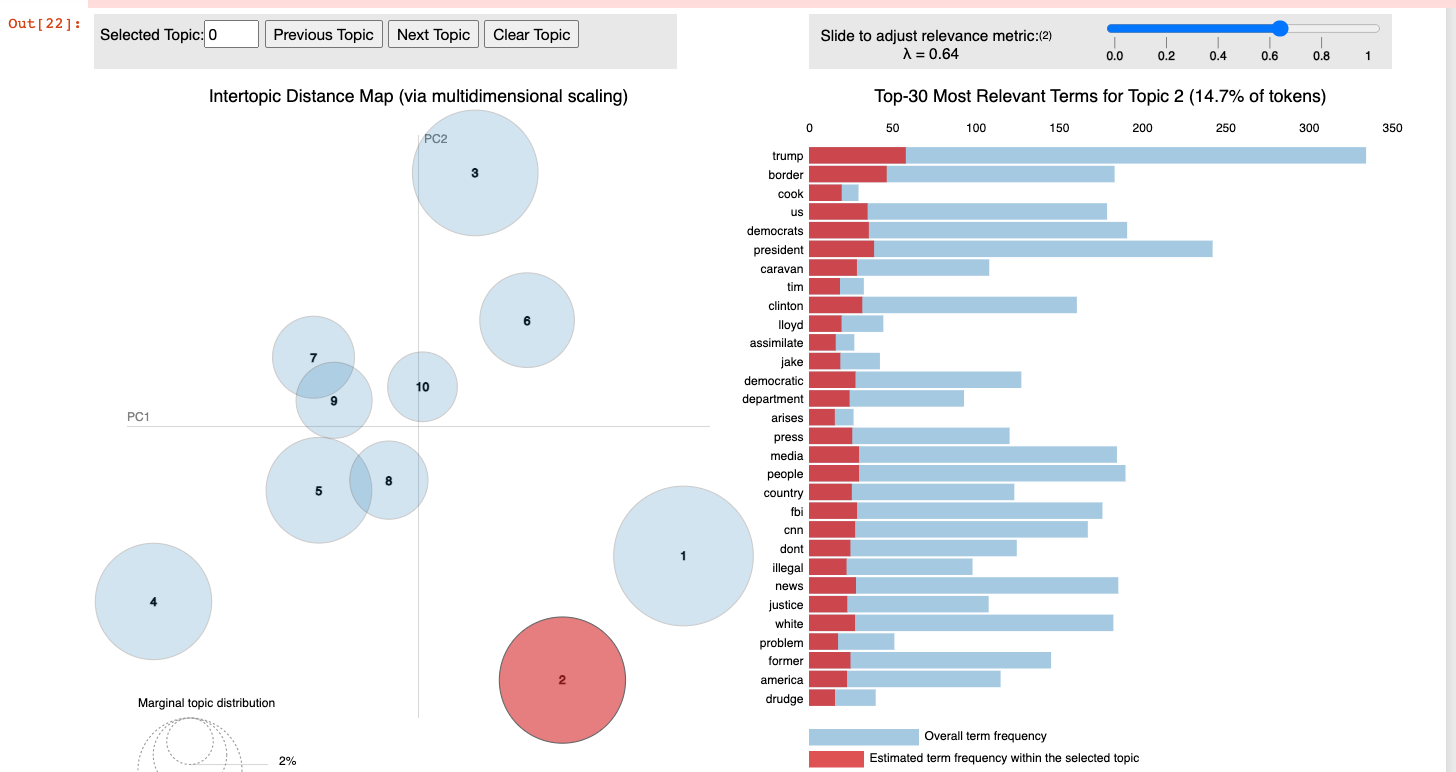
\includegraphics[width=\paperwidth,height=.5\paperheight,keepaspectratio]{../pictures/lda}}
\end{frame}

\iffalse
\begin{frame}{Visualization with pyldavis}
	Short note about the $\lambda$ setting:
	
	It influences the ordering of the words in pyldavis.
	
	\begin{quote}
		``For $\lambda = 1$, the ordering of the top words is equal to the ordering of the standard conditional word probabilities. For $\lambda$ close to zero, the most specific words of the topic will lead the list of top words. In their case study, Sievert and Shirley (2014, p. 67) found the best interpretability of topics using a  $\lambda$-value close to .6, which we adopted for our own case'' (Maier et al., 2018, p.~107)
	\end{quote}
	
	
	\tiny{Maier, D., Waldherr, A., Miltner, P., Wiedemann, G., Niekler, A., Keinert, A., \ldots Adam, S. (2018). Applying LDA Topic Modeling in Communication Research: Toward a Valid and Reliable Methodology. \textit{Communication Methods and Measures, 12}(2--3), 93--118. doi:10.1080/19312458.2018.1430754}
\end{frame}
\fi

\subsection{Choosing the best (or a good) topic model}

\begin{frame}{Choosing the best (or a good) topic model}
	\begin{itemize}
		\item There is no single best solution (e.g., do you want more coarse of fine-grained topics?)
		\item Non-deterministic
		\item Very sensitive to preprocessing choices
		\item Interplay of both metrics and (qualitative) interpretability 
	\end{itemize}
	
	See for more elaborate guidance:
	
	\tiny{Maier, D., Waldherr, A., Miltner, P., Wiedemann, G., Niekler, A., Keinert, A., \ldots Adam, S. (2018). Applying LDA Topic Modeling in Communication Research: Toward a Valid and Reliable Methodology. \textit{Communication Methods and Measures, 12}(2--3), 93--118. doi:10.1080/19312458.2018.1430754}
	
\end{frame}



\begin{frame}{Evaluation metrics}
	\begin{block}{qualitative: human judgement}
	Observation and interpretation based: observe the top N words in your topic, and evaluate the quality of the coherence of the topic.  Can you identify words that do not belong to a topic?
	\end{block}
	
	\pause 
	\begin{block}{quantitative: coherence}
		\begin{itemize}
			\item mean coherence of the whole model: attempts to quantify the interpretability
			\item coherence per topic: allows to get topics that are most likely to be coherently interpreted (\texttt{.top\_topics()})
		\end{itemize}
	\end{block}
	
\end{frame}


\begin{frame}{So, how do we do this?}
	\begin{itemize}[<+->]
		\item Estimate multiple models, store the metrics for each model, and then compare them (numerically, or by plotting)
		\item Idea: We select some candidate models, and then look whether they can be interpreted.
		\item But what can we tune?
	\end{itemize}
\end{frame}


\begin{frame}{Choosing $k$: How many topics do we want?}
	\begin{itemize}
		\item Typical values: $10<k<200$
		\item Too low: losing nuance, so broad it becomes meaningless
		\item Too high: picks up tiny pecularities instead of finding general patterns
		\item There is no inherent ordering of topics
		\item We can throw away or merge topics later, so if out of $k=50$ topics 5 are not interpretable and a couple of others overlap, it still may be a good model
	\end{itemize}
\end{frame}


\begin{frame}[fragile]{Choosing $\alpha$: how sparse should the document-topic distribution $\theta$ be?}
	\begin{itemize}
		\item The higher $\alpha$, the more topics per document 
		\item Default: $1/k$
		\item But: We can explicitly change it, or -- really cool -- even learn $\alpha$ from the data (\texttt{alpha = "auto"})
	\end{itemize}
	
	\pause 
	



\begin{minted}[%
	breaklines,
	linenos,
	fontsize=\tiny,
	frame=single,
	xleftmargin=0pt,]
	{python}
mylda =LdaModel(corpus=tfidfcorpus[ldacorpus], id2word=id2word, num_topics=50, alpha='auto', passes=10)
\end{minted}
	
\end{frame}


\iffalse
\begin{frame}{Choosing $\eta$: how sparse should the topic-word distribution $\lambda$ be?}
	\begin{itemize}
		\item Can be used to boost specific words
		\item Can also be learned from the data 
	\end{itemize}
	
	\pause
Takeaway: Even though you can do \texttt{eta="auto"}, this usually does not help you much.
	
\end{frame}
	Takeaway: It takes longer, but you probably want to learn alpha from the data, using multiple passes:
\fi

% \subsection{Drawbacks of LDA topic models}


\subsection{Using topic models}

\begin{frame}{Using topic models}
	
	You got your model -- what now?
	
	\begin{enumerate}
		\item Assign topic scores to documents
		\item Label topics
		\item Merge topics, throw away boilerplate topics and similar (manually, or aided by cluster analysis)
		\item Compare topics between, e.g., outlets
		\item or do some time-series analysis.
	\end{enumerate}
	
	
	Example:
	\tiny{Tsur, O., Calacci, D., \& Lazer, D. (2015). A Frame of Mind: Using Statistical Models for Detection of Framing and Agenda Setting Campaigns. \textit{Proceedings of the 53rd Annual Meeting of the Association for Computational Linguistics and the 7th International Joint Conference on Natural Language Processing} (pp. 1629–1638).}
	
	
	
\end{frame}



\begin{frame}[plain]
	
	\begin{block}{Exercise for this week's lab session}
		\footnotesize
		\begin{itemize}
			\item Work through the example notebook on LDA: \url{https://github.com/uva-cw-ccs2/2324s2/blob/main/week03/exercise/topic-modelling.ipynb}
			\end{itemize}
	\end{block}
\end{frame}

\section{Recommender Systems}

\begin{frame}
	\makebox[\linewidth]{
		
\includegraphics[width=\columnwidth,height=\paperheight,keepaspectratio]{../pictures/social_media.jpeg}}
\end{frame}
% recommender systems are everywhere around us.

\begin{frame}{Recommender Systems in Communication Science}  
	\begin{block}{New research questions}
		\begin{enumerate}
			\item<2-> \alert{Political communication and journalism}. E.g., to craft personalized news diets. This may have, however, consequences for the diversity of news diets and for democracy \parencite{Moller2018, Locherbach2018}
			\item<3-> \alert{Organizational and corporate communication}. E.g., applications in the field of hiring and recruitment.
			\item<4-> \alert{Persuasive communication}. E.g., in the health domain--recommendation algorithms for tailored health interventions \parencite{Kim2019}
			\item<5-> \alert{Entertainment communication}. E.g., movie recommenders
				\end{enumerate}
	\end{block}
\end{frame}

\begin{frame}{Recommender Systems} 
\begin{block}{Two central problems within Recommender Systems}
	\begin{enumerate}
		\item<2-> \alert{Predicting problem}. Typical problem involves a lot of missing data (e.g., user only rated a small subset of movies/news articles/ etc.) How can we deal with missing data? 
		\item<3-> \alert{Ranking problem}.  Given \textit{n} items, can we identify the top \textit{k} items to recommend?
	\end{enumerate}
\end{block}
\only<4->{These problems are not isolated; rather, they are connected. }
\end{frame}

\begin{frame}{Recommender Systems} 
\begin{block}{How do recommender systems learn?}
	\begin{enumerate}
		\item<2-> \alert{Explicit user preferences}. Ratings or responses 
		\item<3-> \alert{Implicit user preferences}. E.g., clicks or viewing time
		\item<3-> \alert{Content}. E.g., based on text similarity techniques
	\end{enumerate}
\end{block}
\end{frame}

\begin{frame}{Recommender Systems} 
\begin{block}{Types of recommender systems  \parencite{Wieland2021, Locherbach2018, Moller2018}}
	\begin{enumerate}
		\item 'Basic' knowledge-base recommender systems
		\item Content-based recommender systems
		\item Collaborative  recommenders 
	\end{enumerate}
\end{block}{\tiny }
\end{frame}

\section[Knowledge-based RecSys]{Knowledge-based Recommender Systems}
\begin{frame}{Knowledge-based recommender system} 
\begin{block}{When to use?}
	\begin{itemize}
		\item<2-> To overcome the \textbf{cold start problem}; when we do not have ratings of individual users. 
		\item<3-> Simple model. It does not rely on user's explicit or implicit ratings, but on specific queries.
		\item<4-> Typical use case: Real-estate. Buying a house is, for most families, a rare/ single event. 
	\end{itemize}
\end{block}
\end{frame}

% This prints the bibliography on the slide
%\section{An example with some Python code\dots}

\begin{frame}
\makebox[\linewidth]{
	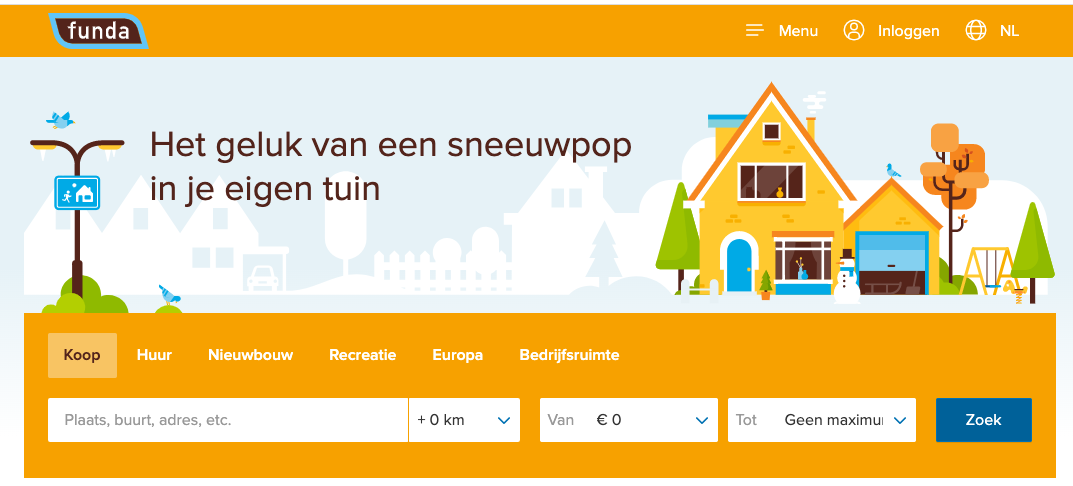
\includegraphics[width=\columnwidth,height=\paperheight,keepaspectratio]{../pictures/funda}}
\end{frame}

\begin{frame}{Use case: ImDb database}
\makebox[\linewidth]{
	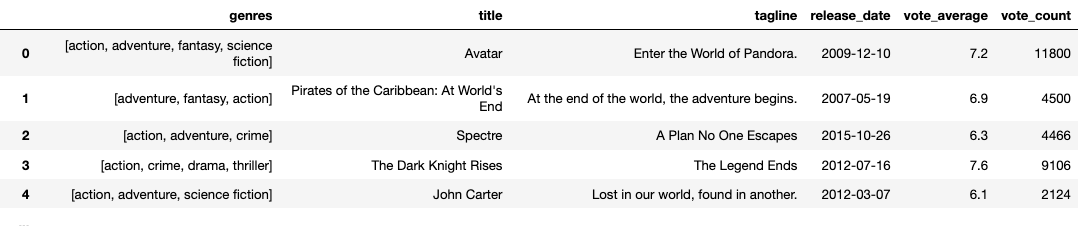
\includegraphics[width=\columnwidth,height=\paperheight,keepaspectratio]{../pictures/data}}
\end{frame}

\question{What are relevant variables to use in a knowledge-based recommender system?}

\begin{frame}[fragile]{Knowledge-based recommender system}
How can we work with user input without a front-end (such as the website of funda? 
\pause
$\rightarrow$ enter python's native \alert{input()} function.
\pause
\begin{minted}{python}
print("What is your favorite movie genre?")
genre = input()
\end{minted}
\pause
\begin{lstlistingoutput}
what is your favorite movie genre?
[...]
\end{lstlistingoutput}
\end{frame}


\begin{frame}[fragile]{Improving knowledge-based recommender system}
\begin{block}{When to use?}
	\begin{itemize}
		\item <1-> It is important to think about ways to make the recommendation relevant for individuals
		\item <2-> Do you have more information in your db that make your top-listed recommendations as relevant as possible?
	\end{itemize}
\end{block}
\pause
\begin{minted}[fontsize=\footnotesize]{python}
recommend_movies = movies.sort_values('vote_average', ascending=False)
\end{minted}
\end{frame}

\section[Content-based RecSys]{Content-based Recommender Systems}

\begin{frame}
	\begin{block}{Content-based systems}
		\begin{itemize}
			\item <1-> Recommends items based on user's profiles. 
			\item <2-> Profiles are based on e.g., ratings, and represents user's tasts/ preferences. 
			\begin{itemize}
				\item <3-> For example, how often a user has clicked on, or liked, a movie. 
			\end{itemize}
			\item <4-> Recommendation is based on \alert{similarity} beween items in the content.
			\begin{itemize}
				\item <5-> Content is here: e.g., genre, tags, plot, authors, directors, location, etc. 
			\end{itemize}
		\end{itemize}
	\end{block}
\end{frame}

\begin{frame}{Example of a content-based recsys}
	\makebox[\linewidth]{
		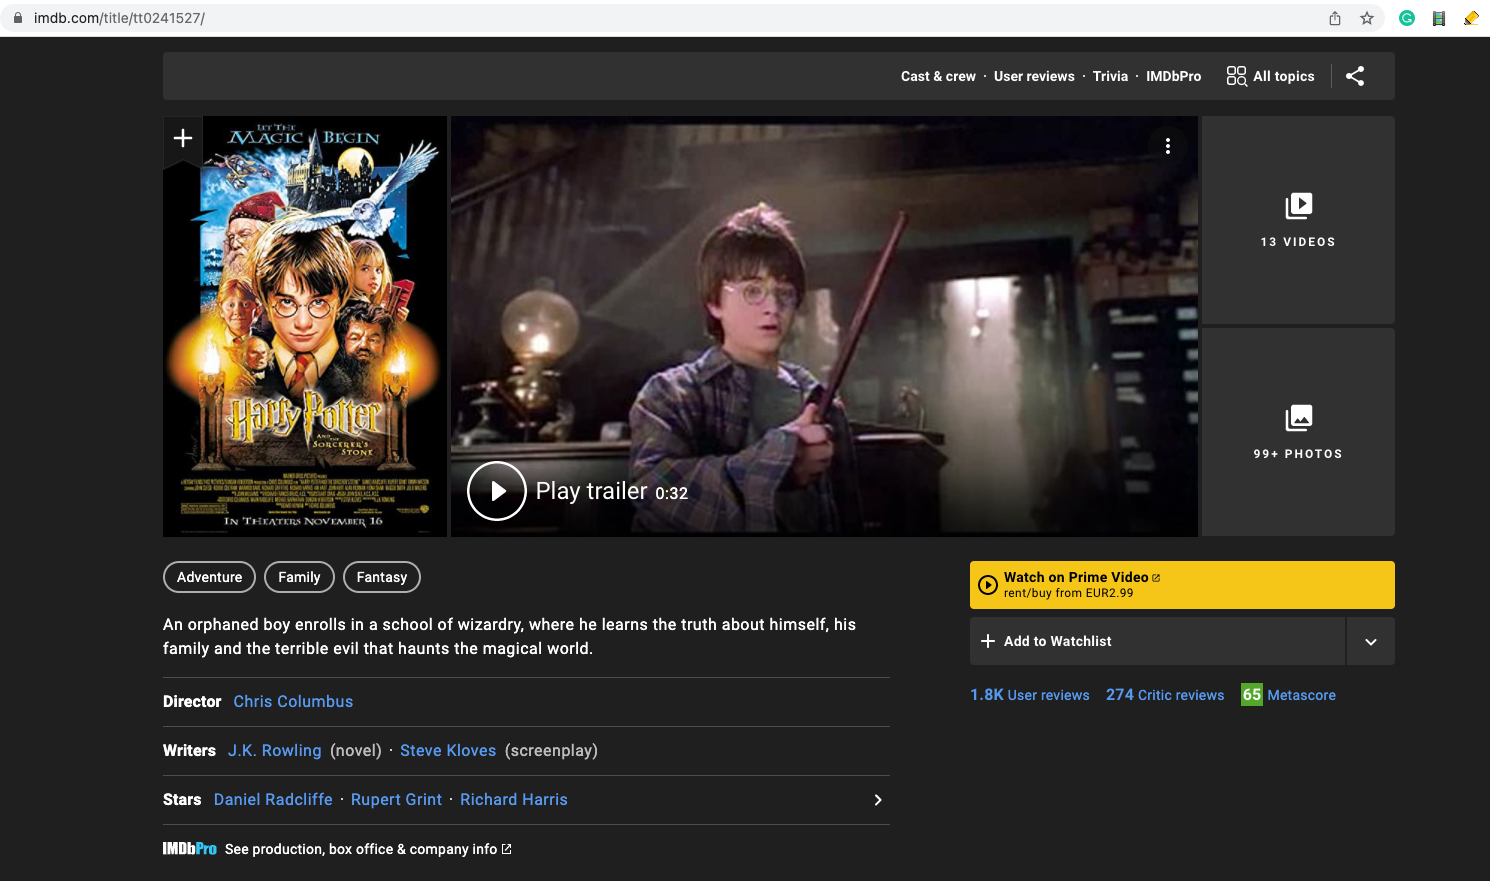
\includegraphics[width=\columnwidth,height=\paperheight,keepaspectratio]{../pictures/harry1.png}}
\end{frame}

\begin{frame}{Example of a content-based recsys}
	\makebox[\linewidth]{
		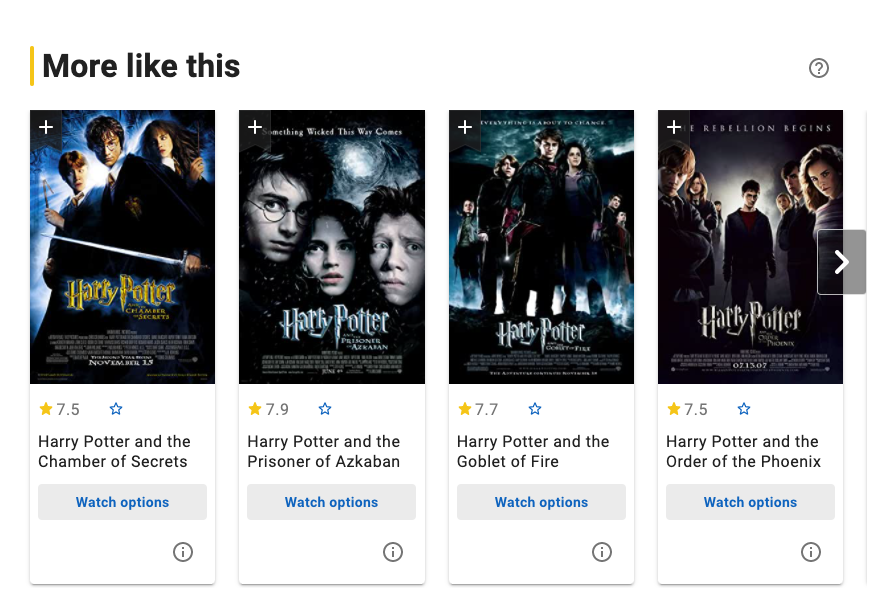
\includegraphics[width=\columnwidth,height=\paperheight,keepaspectratio]{../pictures/harry2.png}}
\end{frame}

%as you can see, it works quite well, but also has its drawbacks.. can be quite obvious.

%using information of the items themselves, rather than the aggregate user data. Even for more advanced recommender systems, baking in some knowledge about the content can be very helpful. 

%The movielens dataset does not give us a lot of information, but it does 

%Let's have a look again at the MovieLens dataset. If we know given user likes a specific genre, the user might also like other genres. In addition, we can use year of release. We can narrow it down further to movies that are close to a specific release data. 
% there is all sort of information availabe here, that we might use. 

\begin{frame}{Use case: ImDb database}
	Let's have a look at our use case again. \\
	Are there attributes that you could use to estimate similarity in movies?
	\makebox[\linewidth]{
		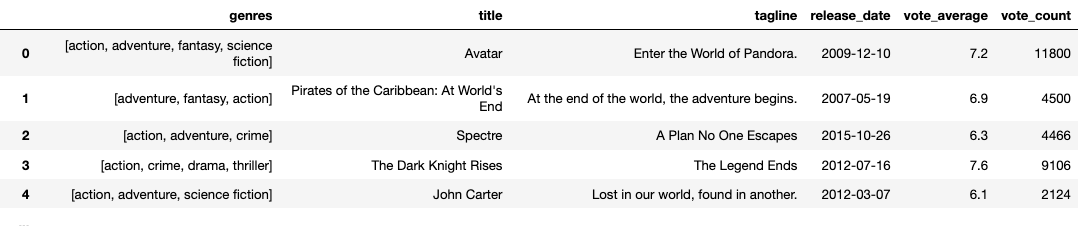
\includegraphics[width=\columnwidth,height=\paperheight,keepaspectratio]{../pictures/data}}
\end{frame}

% how can we calculate similarity, just based on genre?
% Cosine is very handy, not only for textule data, but also for different types of numeric data. 

% to make it easier to understand, lets imagine that every movie has only one of the follwoing genres: 
%romance or comedy

\begin{frame}{Similarity between movies}
	\makebox[\linewidth]{
		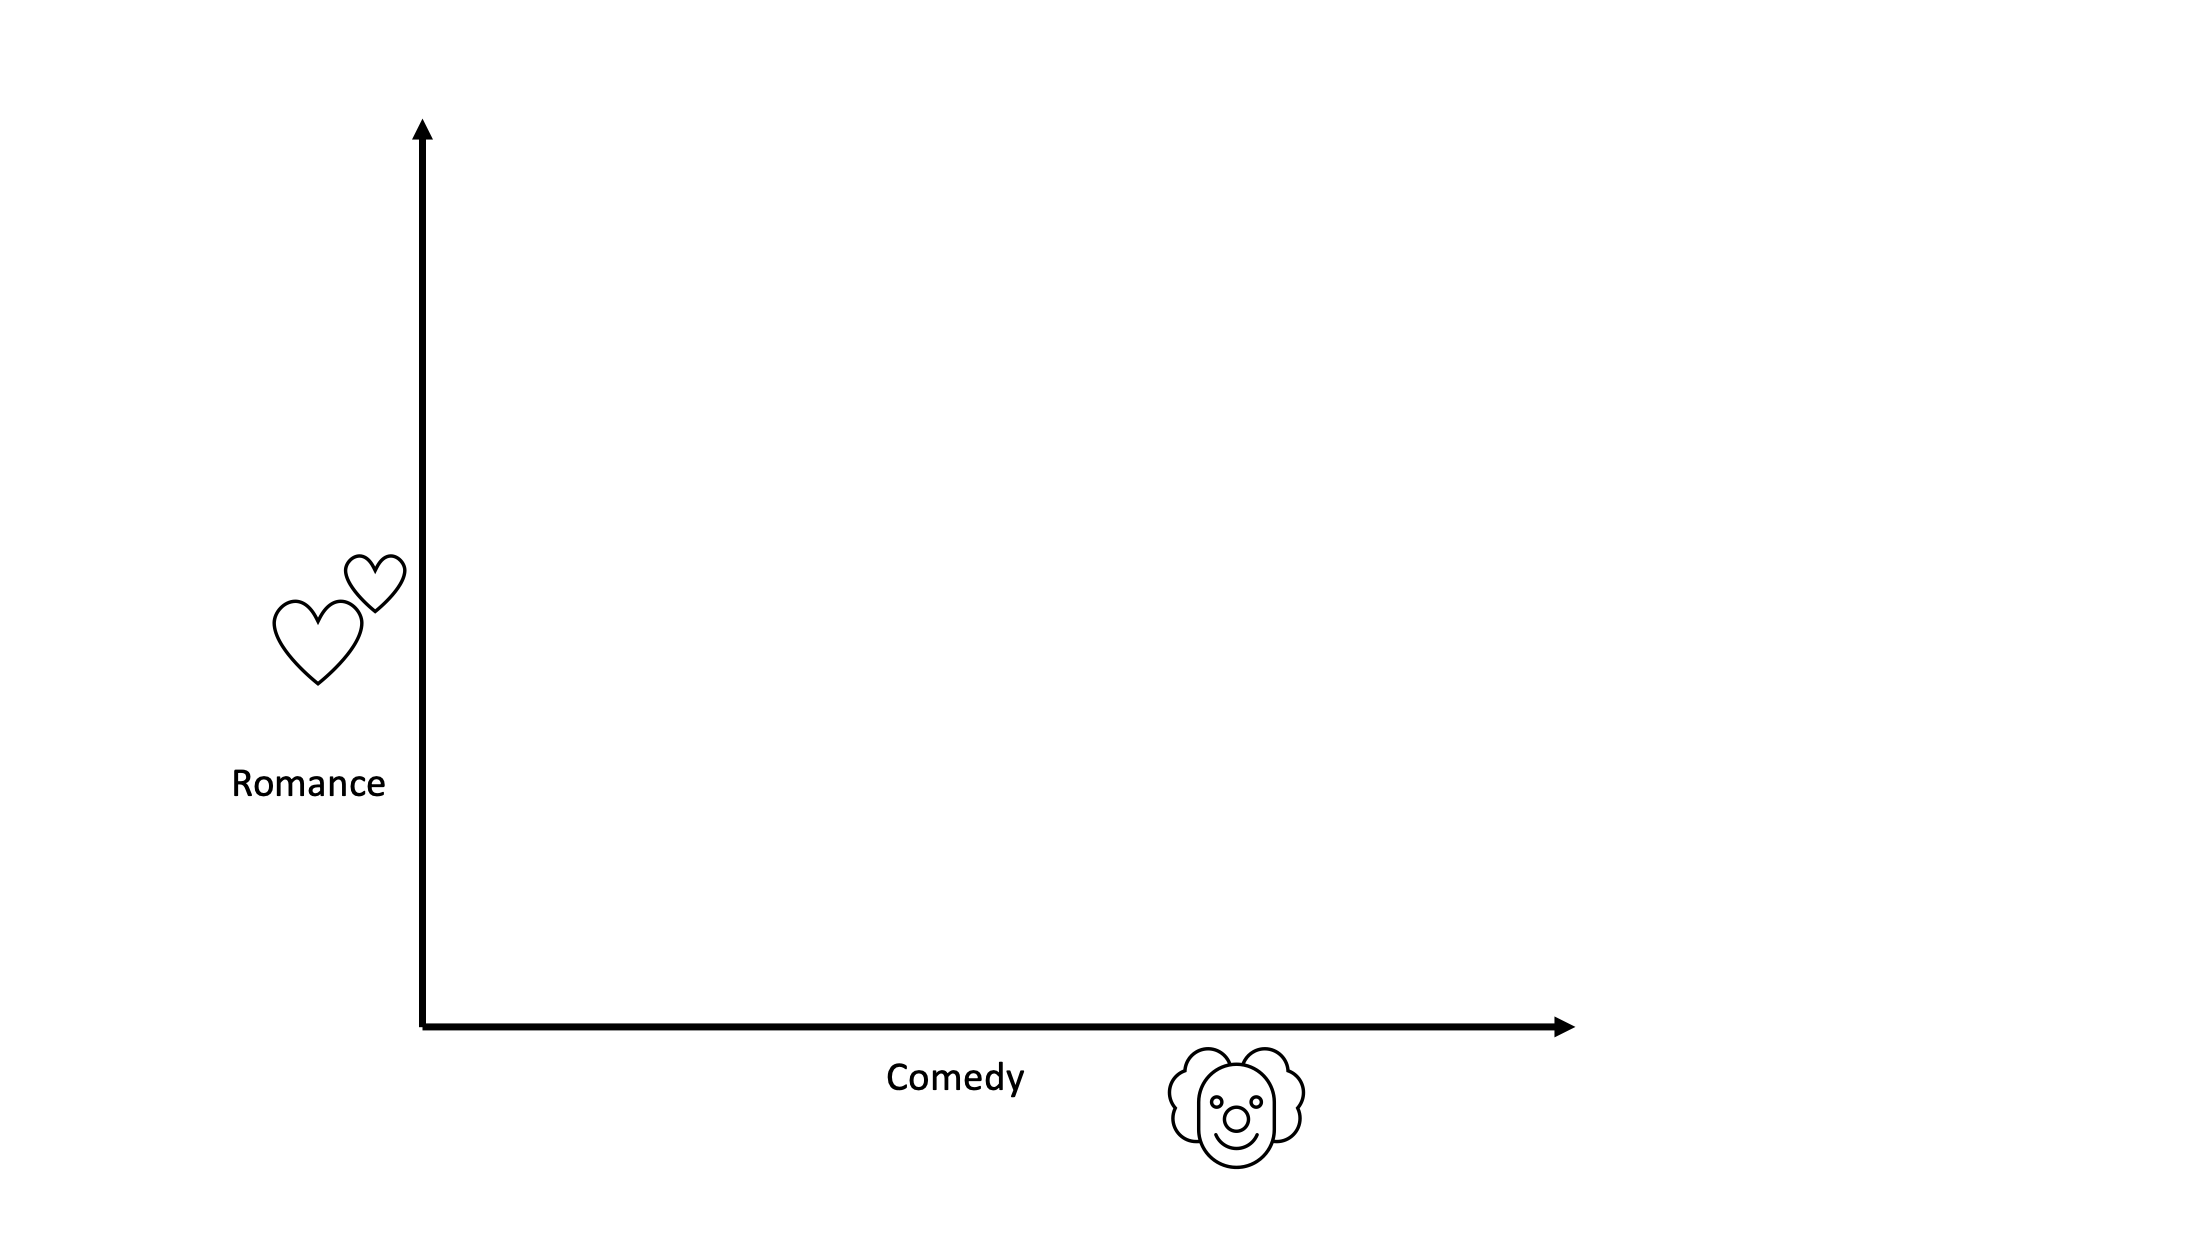
\includegraphics[width=\columnwidth,height=\paperheight,keepaspectratio]{../pictures/Slide1.png}}
\end{frame}

\begin{frame}{Similarity between movies}
	\makebox[\linewidth]{
		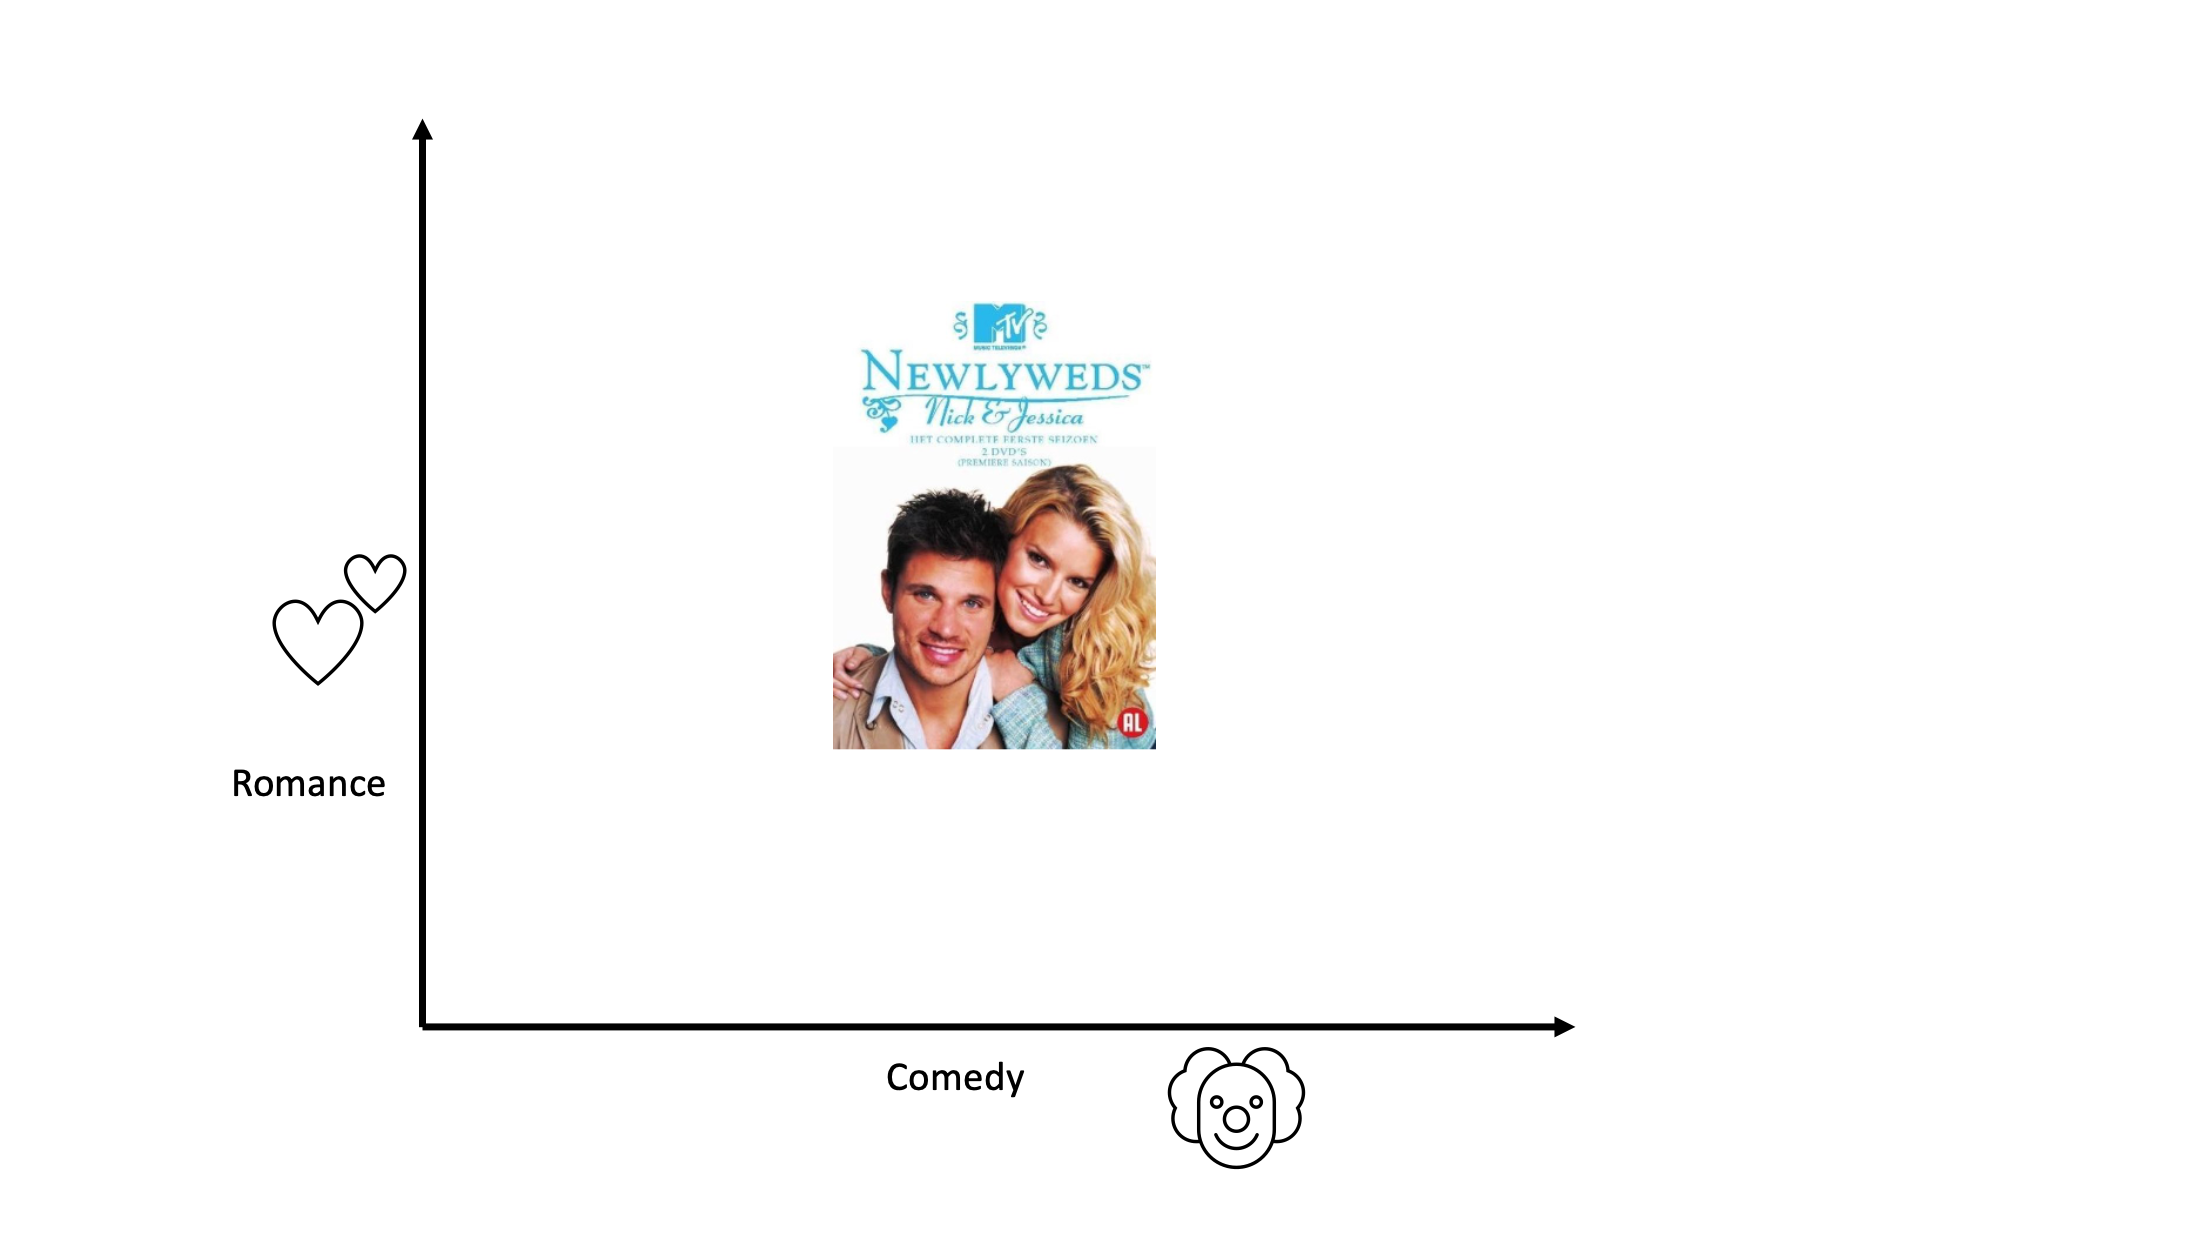
\includegraphics[width=\columnwidth,height=\paperheight,keepaspectratio]{../pictures/Slide2.png}}
\end{frame}

\begin{frame}{Similarity between movies}
	\makebox[\linewidth]{
		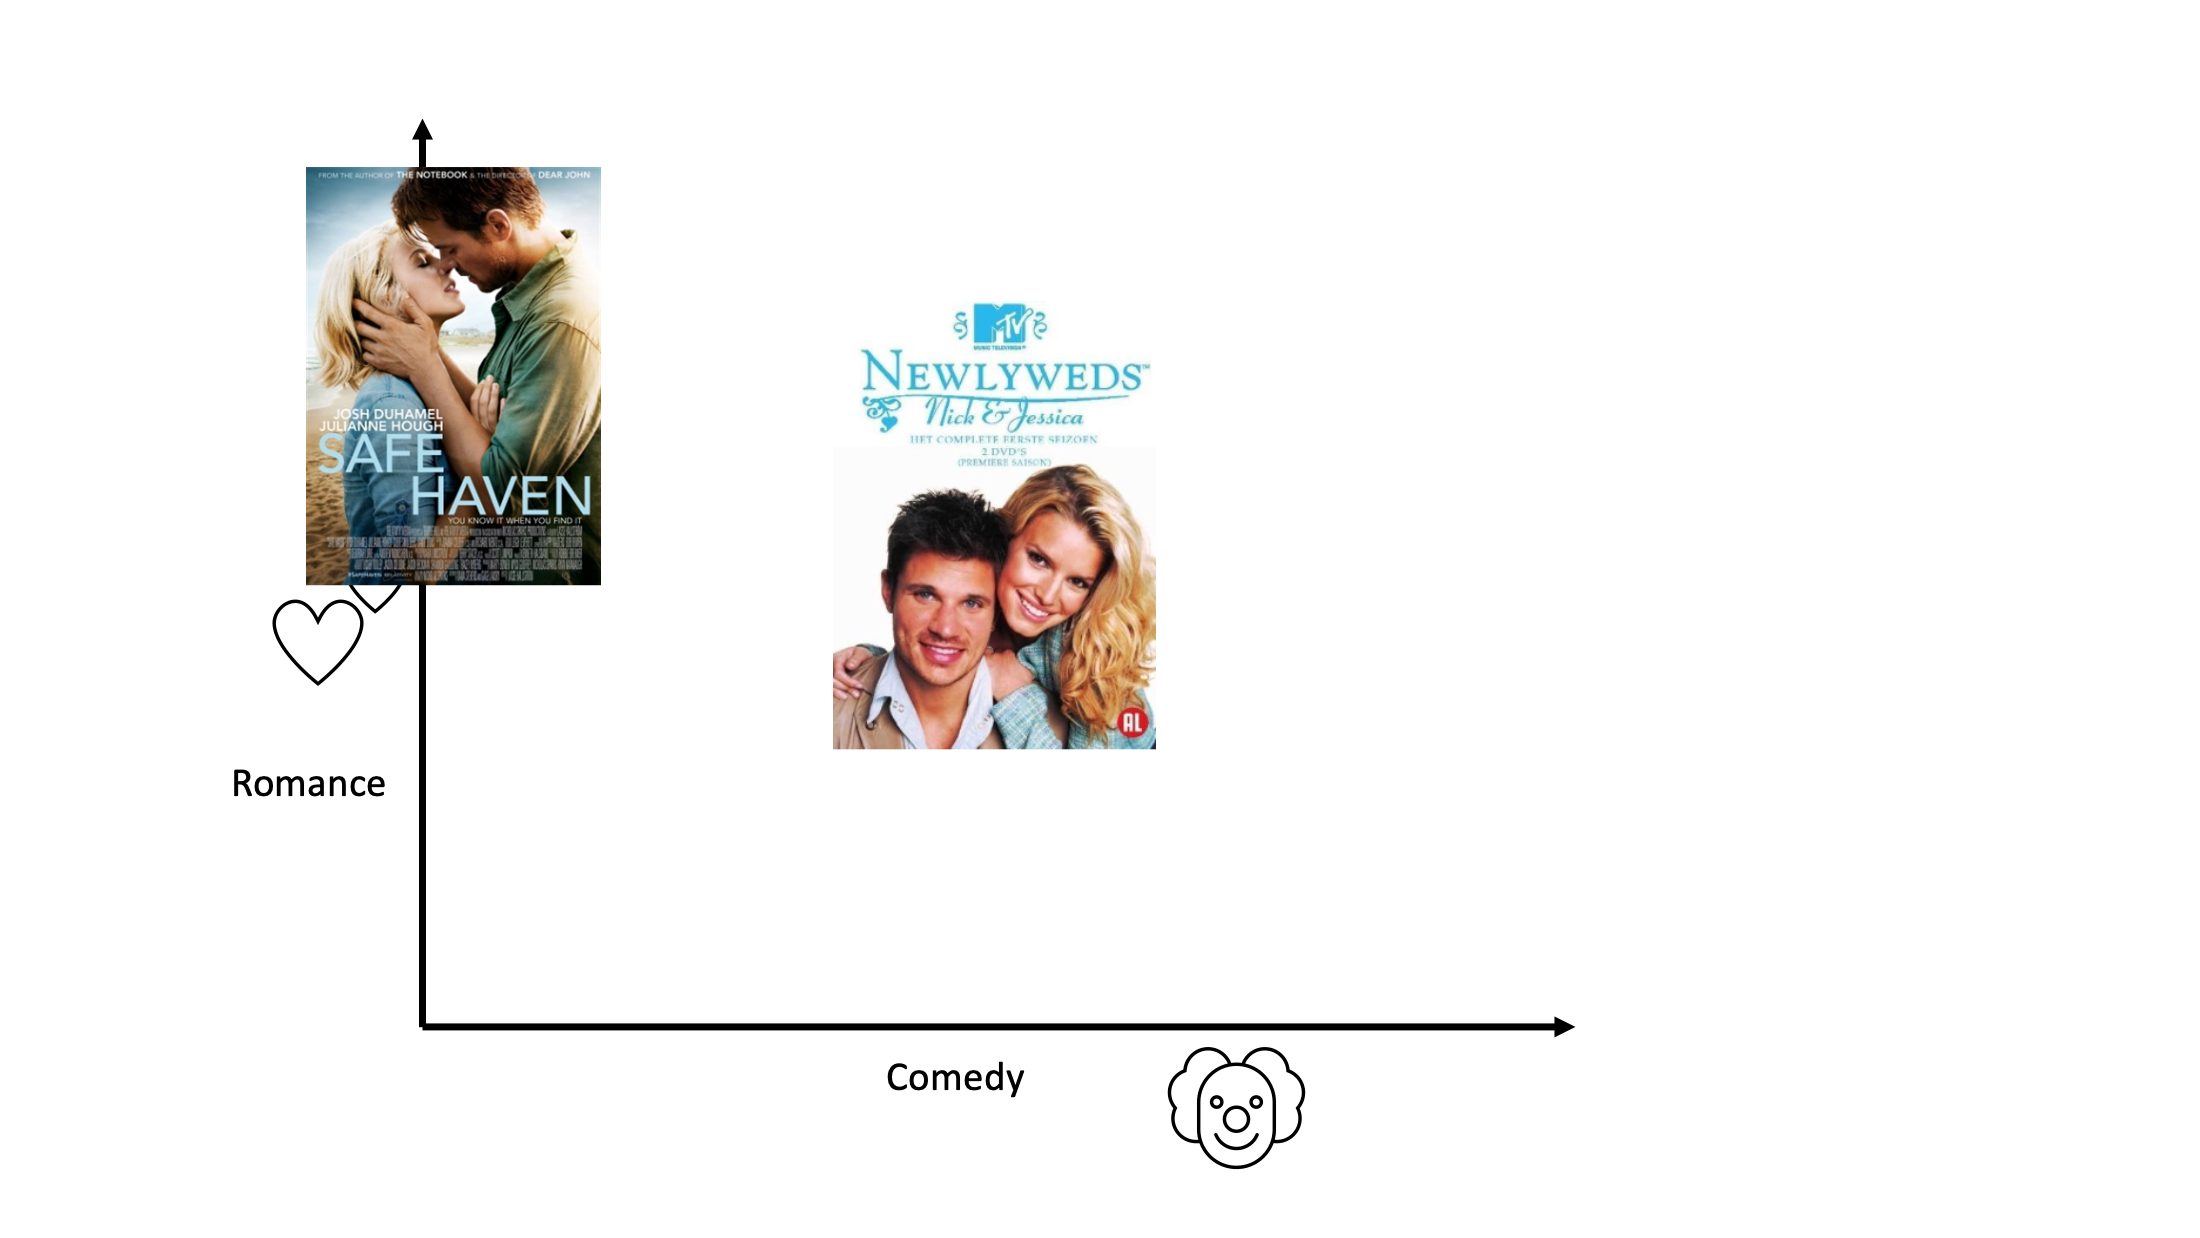
\includegraphics[width=\columnwidth,height=\paperheight,keepaspectratio]{../pictures/Slide3.png}}
\end{frame}

\begin{frame}{Similarity between movies}
	\makebox[\linewidth]{
		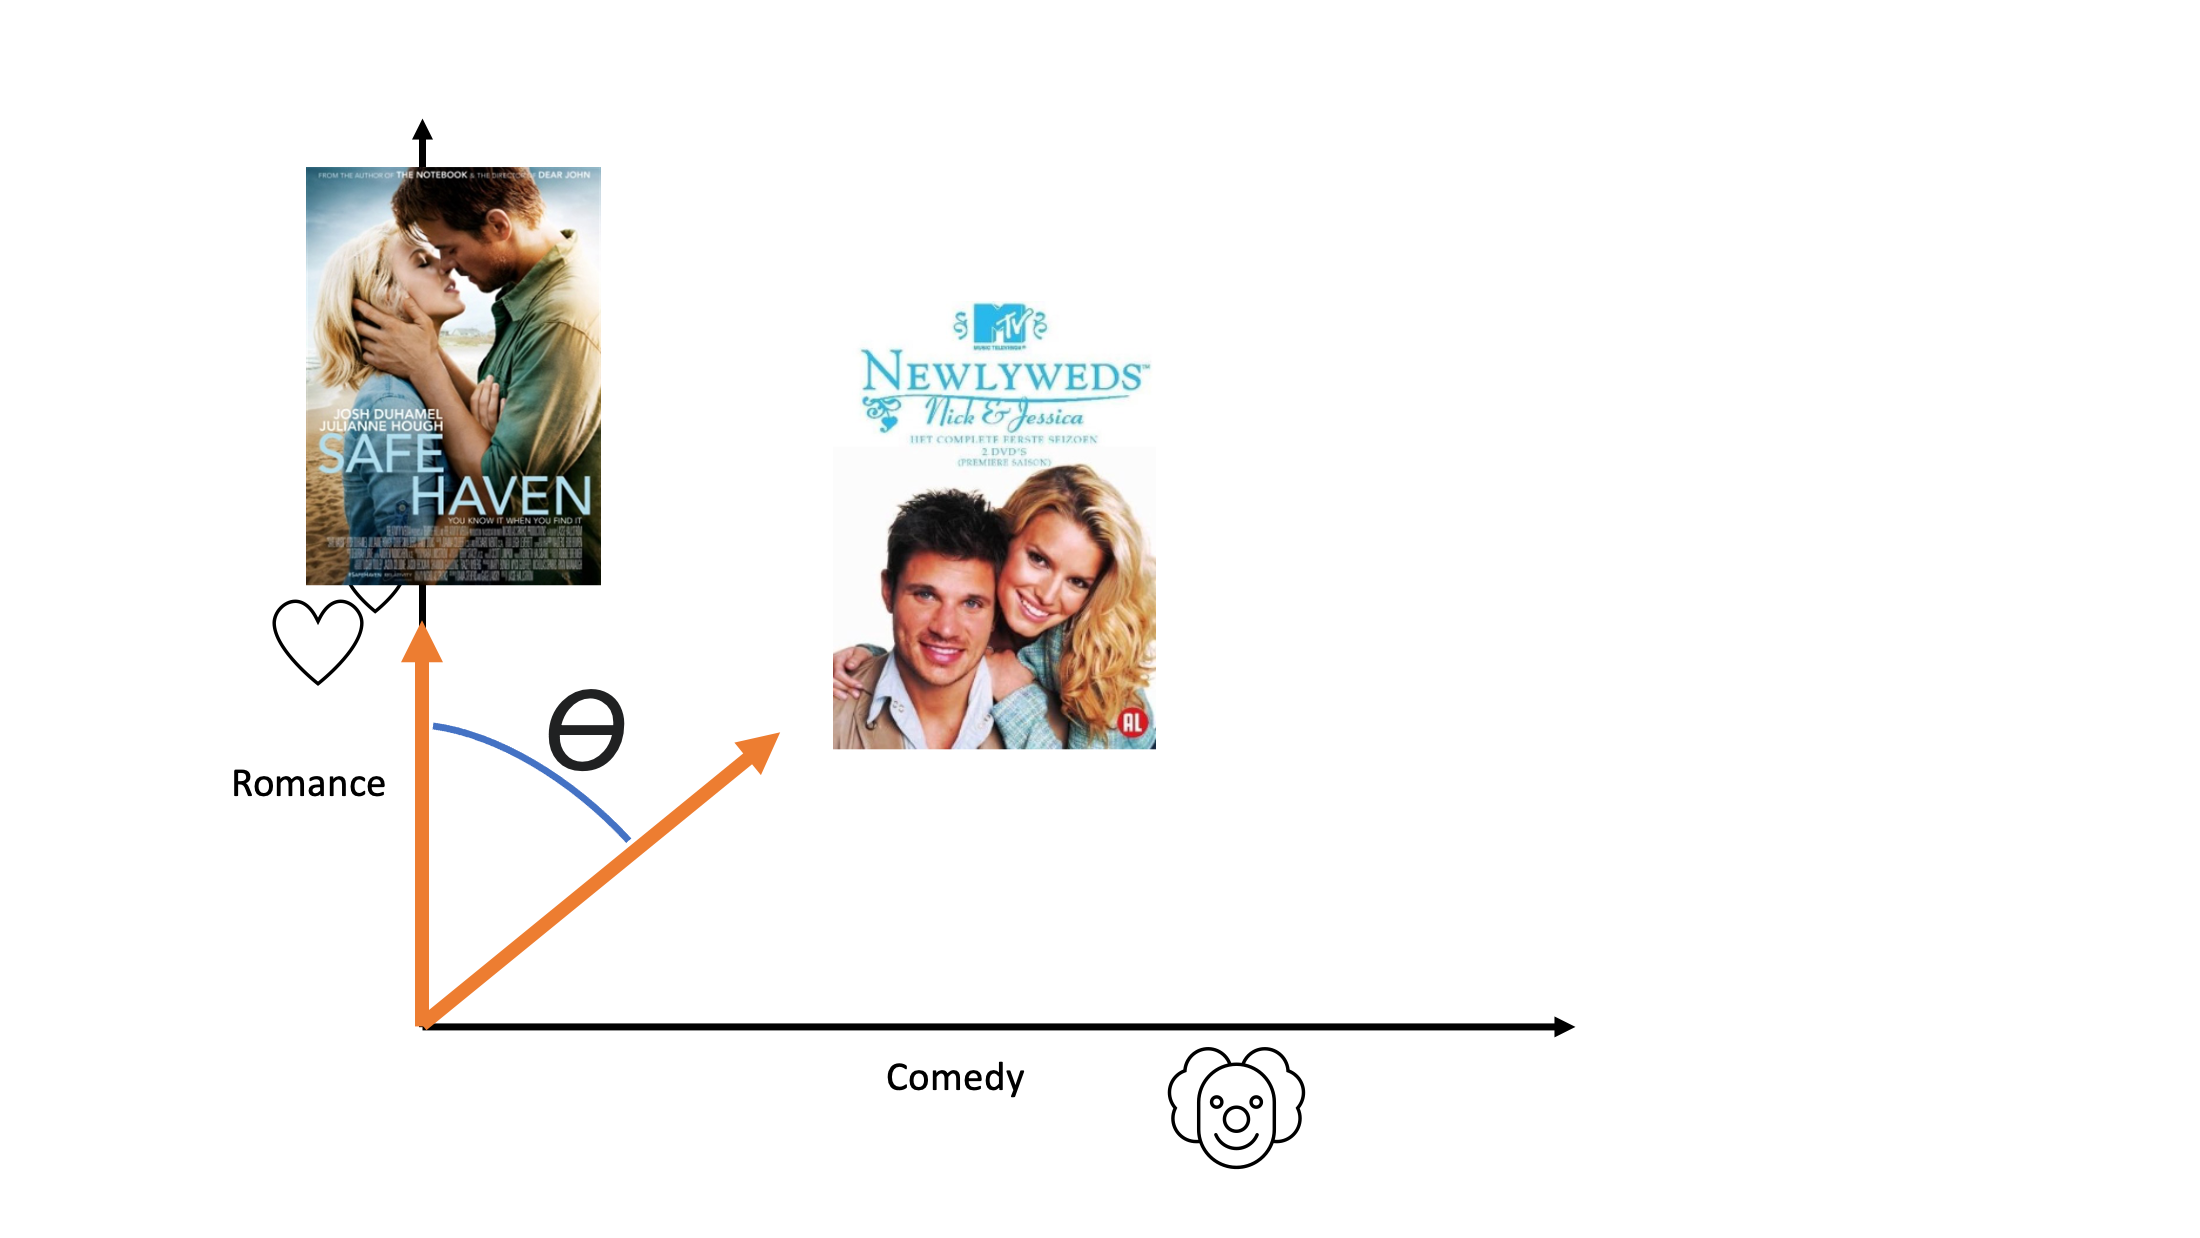
\includegraphics[width=\columnwidth,height=\paperheight,keepaspectratio]{../pictures/Slide4.png}}
\end{frame}

\begin{frame}{Similarity between movies}
	\makebox[\linewidth]{
		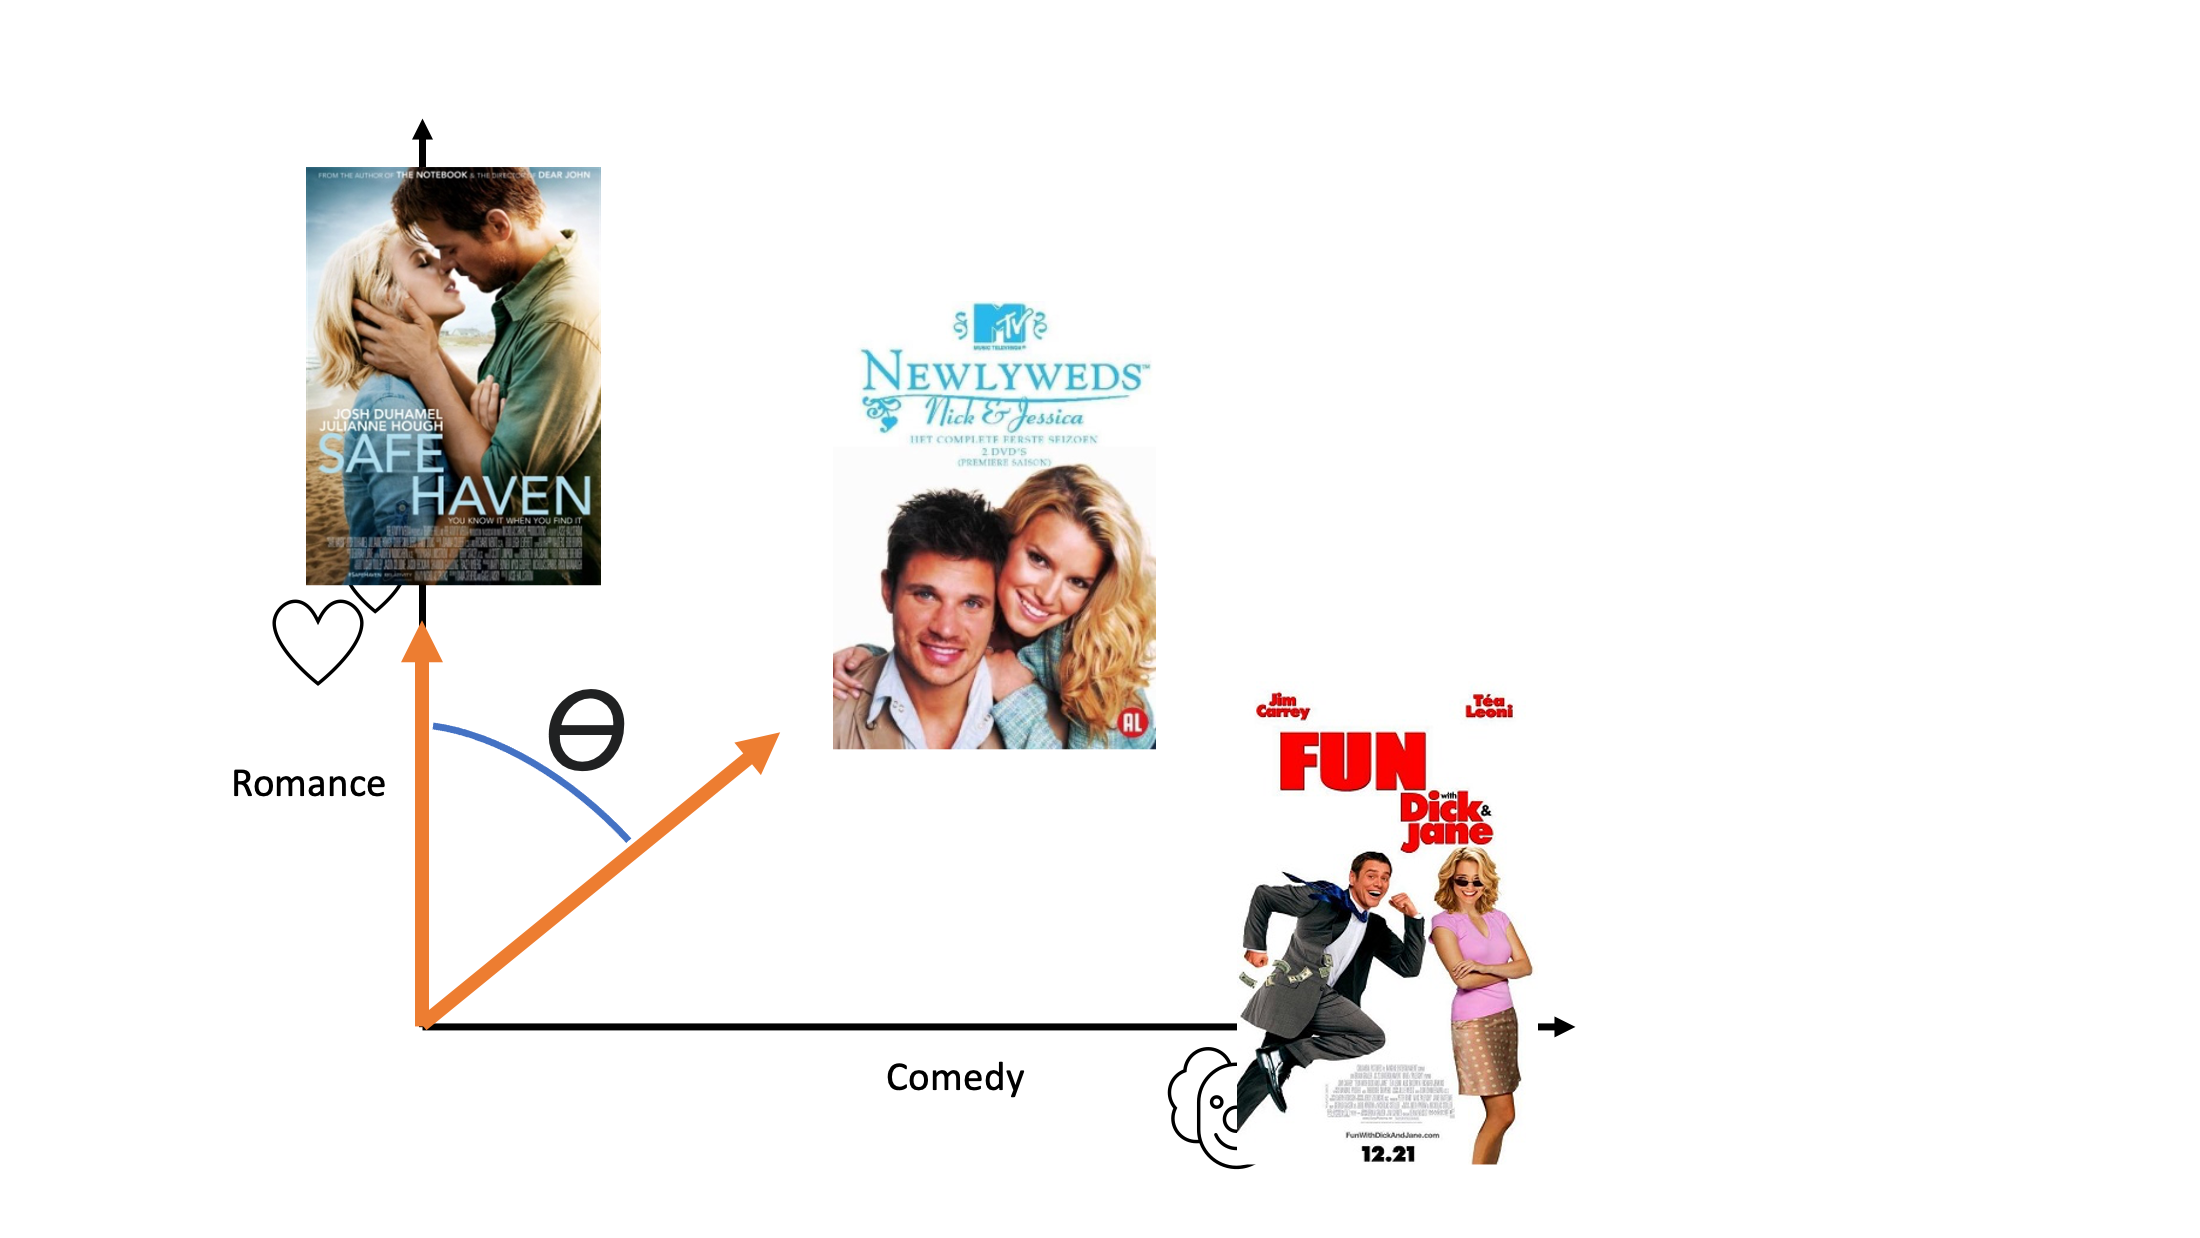
\includegraphics[width=\columnwidth,height=\paperheight,keepaspectratio]{../pictures/Slide5.png}}
\end{frame}

\begin{frame}[fragile]{Let's put this in code!}
	\pause
	First, create a create a toy dataset.
	\pause
	\begin{minted}{python}
data = data.sample(6)
data[['title', 'genres']]
	\end{minted}
	\pause
	\makebox[\linewidth]{
		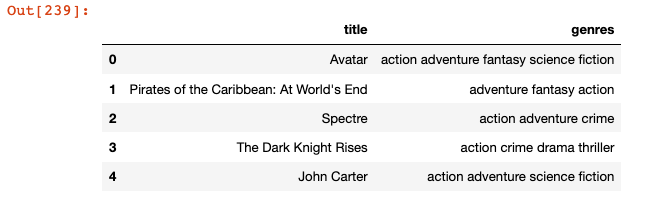
\includegraphics[width=\columnwidth,height=\paperheight,keepaspectratio]{../pictures/toy}}
\end{frame}

\begin{frame}[fragile]{Feature selection and vectorization}
	Let's assume we want to calculate similiarity based on genres. Therefore, we need to vectorize this column. 
	\begin{minted}{python}
tfidf = TfidfVectorizer(stop_words='english')
tfidf_matrix = tfidf.fit_transform(data['genres'])
	\end{minted}
	\pause
Note that we use \alert{tfidf vectorizer} here, but we you might opt for a different one. 
\end{frame}

\begin{frame}[fragile]{Calculate similiarity}
	Now, let's calculate cosine similarity scores between the genre attributes of the movies
	\begin{minted}{python}
from sklearn.metrics.pairwise import cosine_similarity
sim = cosine_similarity(tfidf_matrix)
	\end{minted}
	\pause
This returns an array of the similiarity scores between each movie and all other movies. 
\end{frame}

\begin{frame}[fragile]{Cosine Similairity}
	Let's inspect the output...
\begin{minted}[fontsize=\tiny]{python}
print(sim)
[[1.         0.34503493 0.         0.         0.40824829 0.        ]
[0.34503493 1.         0.16581288 0.         0.28171984 0.29130219]
[0.         0.16581288 1.         0.25964992 0.         0.56921261]
[0.         0.         0.25964992 1.         0.44115109 0.4561563 ]
[0.40824829 0.28171984 0.         0.44115109 1.         0.        ]
[0.         0.29130219 0.56921261 0.4561563  0.         1.        ]]
\end{minted}
\end{frame}


\begin{frame}[plain]
\makebox[\linewidth]{
		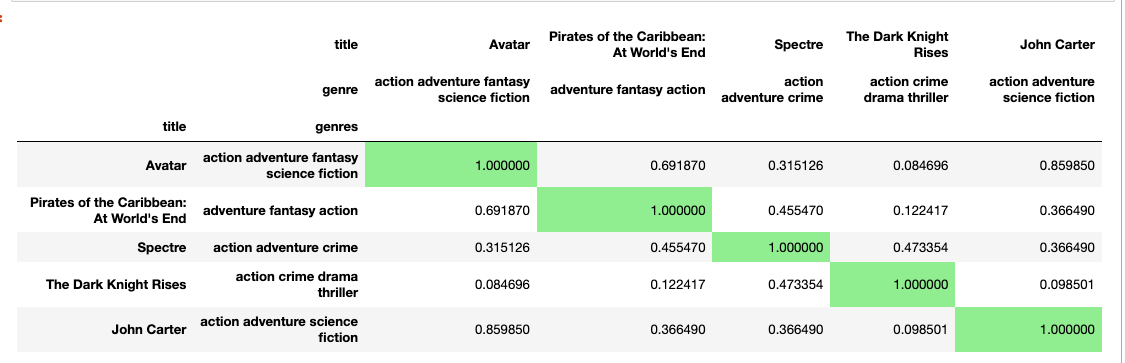
\includegraphics[width=\columnwidth,height=\paperheight,keepaspectratio]{../pictures/cosine_sim}}
	\pause
	Based on this overview, you may assume that users that like \textit{Avatar}, may be interested in \textit{John Carter}. 
		\pause
	\footnotesize{If you want to convert output of \alert{cosine\_similarity} to a \alert{df} type of object, see here \url{https://github.com/uva-cw-ccs2/2223s2/blob/master/week04/exercise/cosine_to_df.md}.}
\end{frame}

\question{Can we automate this proces? Can we automatically find the entry with the most similar movie?}

\subsection*{A more realistic use case}

\begin{frame}{Example of a content-based recsys}
	\makebox[\linewidth]{
		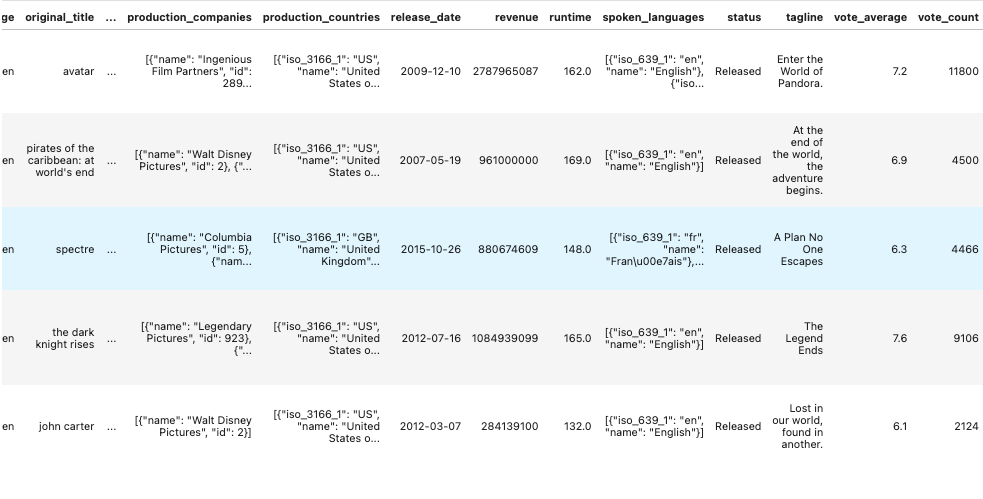
\includegraphics[width=\columnwidth,height=\paperheight,keepaspectratio]{../pictures/dataframe-features}}
\pause
What are interesting features that you can use to base your recommendation on?
\end{frame}


\begin{frame}[fragile]{Get the most similar movies}
First, create an array of cosine scores 
\begin{minted}[%
		breaklines,
		linenos,
		fontsize=\scriptsize,
		frame=single,
		xleftmargin=0pt,]
		{python}
data['combined_features'] = data[['original_title', 'genres', 'overview', 'tagline']].apply(lambda x: ','.join(x.dropna().astype(str)),axis=1)
tfidf = TfidfVectorizer(stop_words='english')
tfidf_matrix = tfidf.fit_transform(data['combined_features'])
cosine_sim = cosine_similarity(tfidf_matrix)
\end{minted}
	\pause
Let's say we want to find the similarity scores associated with the movie \texttt{The Dark Night Rises}. 
\end{frame}

\begin{frame}{Example of a content-based recsys}
	\makebox[\linewidth]{
		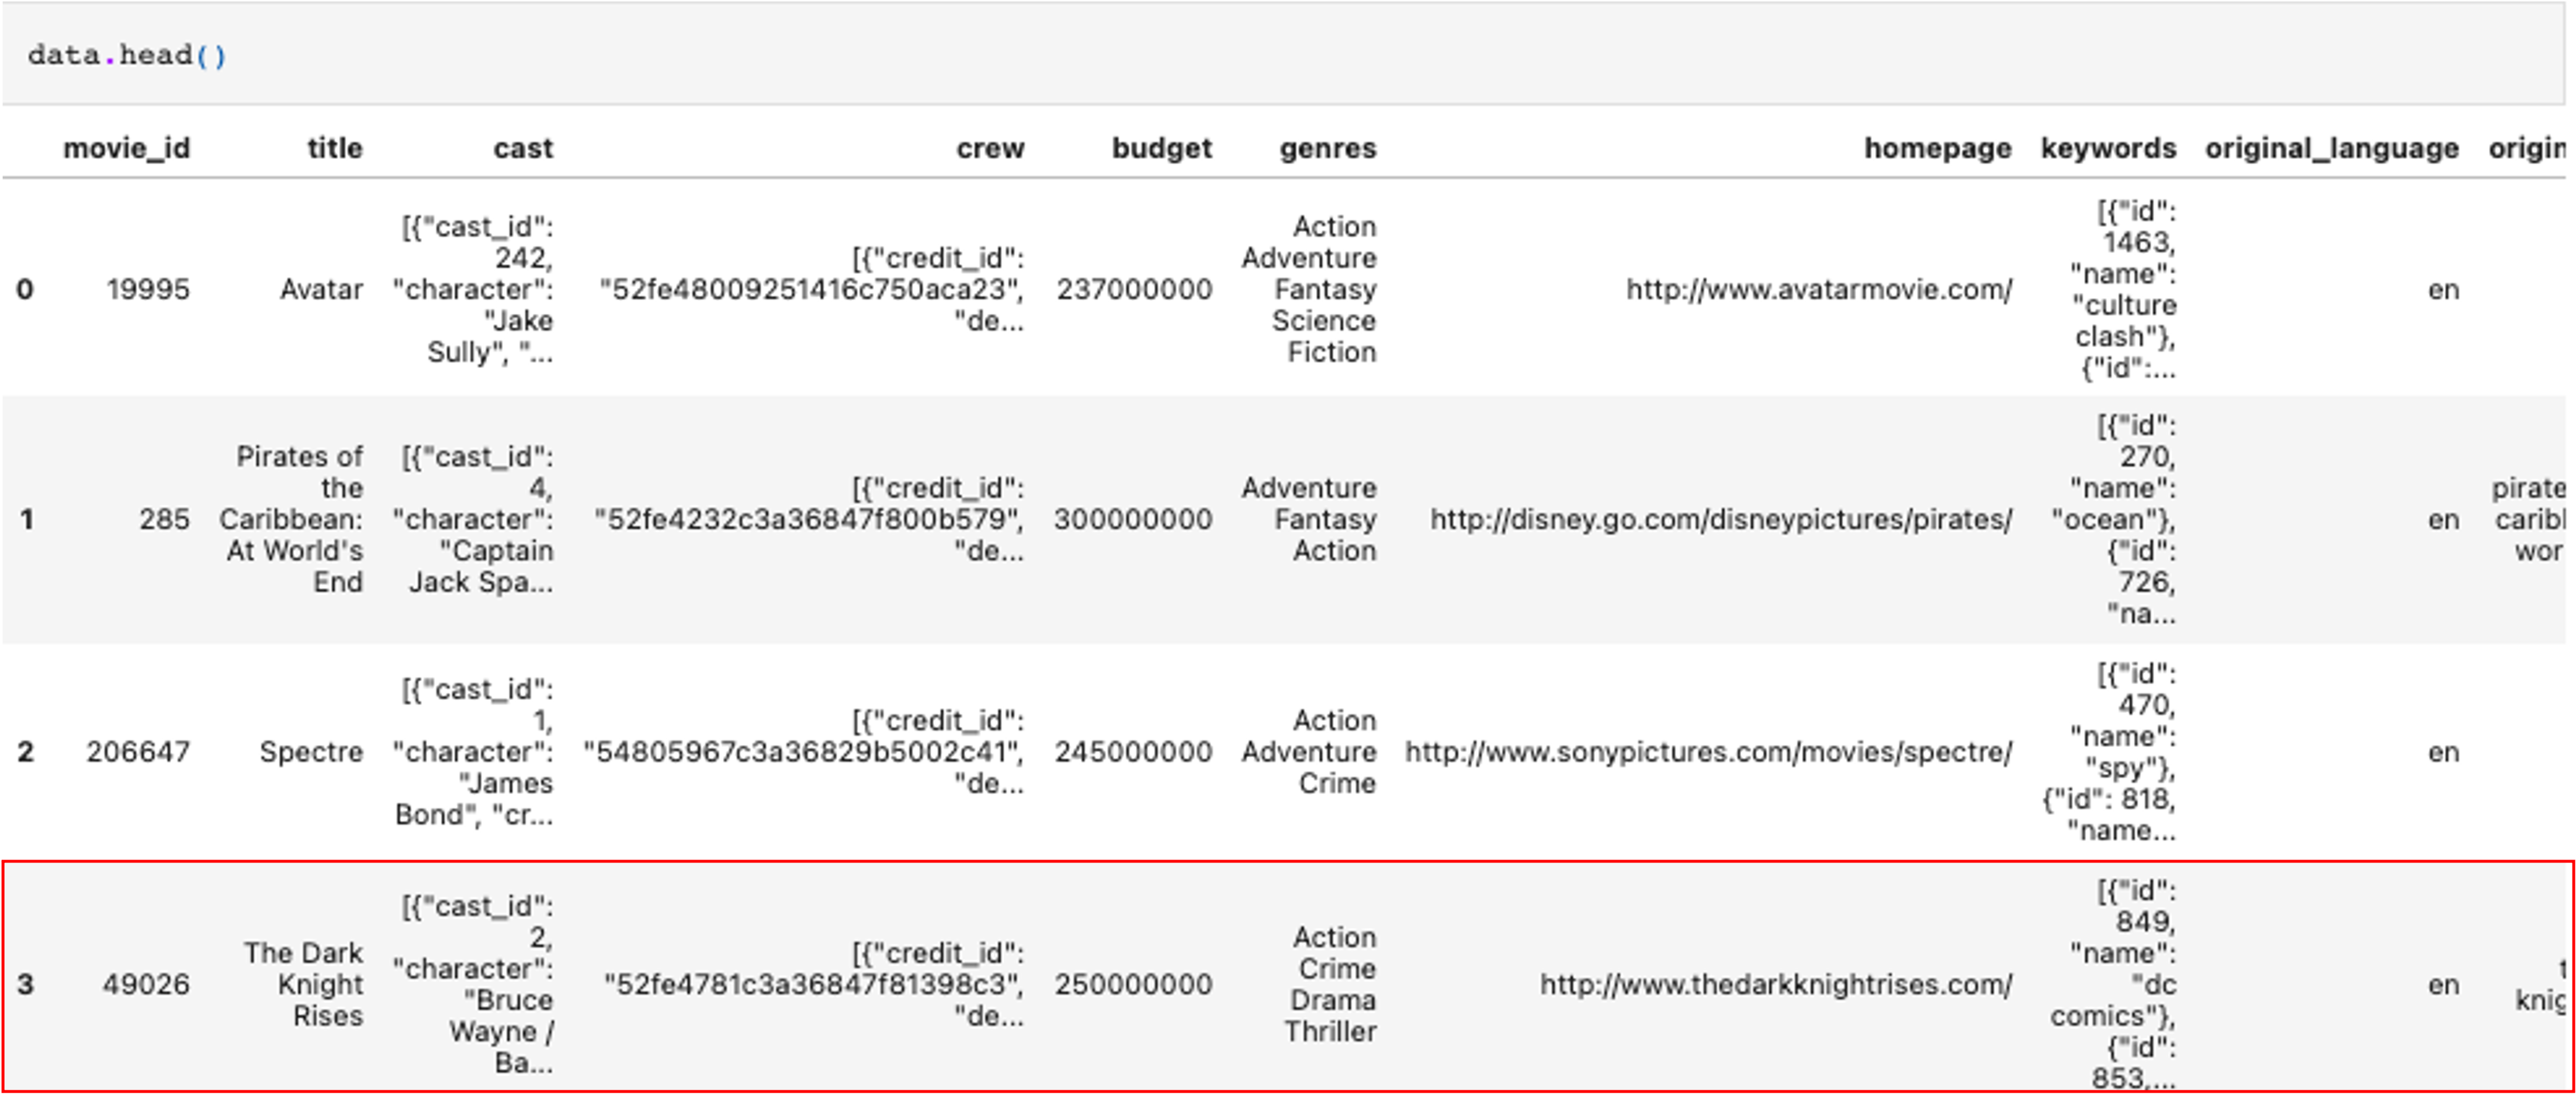
\includegraphics[width=\columnwidth,height=\paperheight,keepaspectratio]{../pictures/df-movies}}
Let's say we want to find the similarity scores associated with the movie \texttt{The Dark Night Rises}. Just by looking at the dataframe, we know it is at index \texttt{3}.
\end{frame}


\begin{frame}[fragile]
\begin{minted}[%
	breaklines,
	linenos,
	fontsize=\scriptsize,
	frame=single,
	xleftmargin=0pt,]
	{python}
cosine_sim[3]
\end{minted}
\pause
\begin{minted}[fontsize=\tiny]{python}
array([0.02331349, 0.00399197, 0.00780174, ..., 0.02860083, 0.03756737, 0.018984  ])
\end{minted}
\pause
A more systematic way to get the index value, is to simple look it up:
\begin{minted}[%
	breaklines,
	linenos,
	fontsize=\scriptsize,
	frame=single,
	xleftmargin=0pt,]
	{python}
indices = pd.Series(data.index, index = data['original_title'])
index = indices['the dark knight rises']
print(index)
\end{minted}
\pause
\begin{minted}[fontsize=\tiny]{python}
3	
\end{minted}
\end{frame}

\begin{frame}[fragile]{Get the most similar movies}
\begin{itemize}
	\item<1->Next, we need to sort the associated vector of cosine similarity scores for this movie to get the most similair movies.
	\item<2->Before sorting the cosine scores, we map the movie-index to the cosine value. We can do so by simple enumerating the cosine scores:
\end{itemize}
\pause
\begin{minted}[%
	breaklines,
	linenos,
	fontsize=\scriptsize,
	frame=single,
	xleftmargin=0pt,]
	{python}
sim_scores = list(enumerate(cosine_sim[index])) 
\end{minted}
\pause
\begin{minted}[fontsize=\tiny]{python}
[(0, 0.023313489832942038),
(1, 0.003991972883233364),
(2, 0.007801739082093903), ...
\end{minted}
\pause
Next, we can simple sort the cosine scores:
\begin{minted}[%
	breaklines,
	linenos,
	fontsize=\scriptsize,
	frame=single,
	xleftmargin=0pt,]
	{python}
sim_scores = sorted(sim_scores, key=lambda x: x[1], reverse=True)
sim_scores = sim_scores[1:11]
\end{minted}
\pause
\begin{minted}[fontsize=\tiny]{python}
[(3, 0.9999999999999998),
(65, 0.3484608502957436),
(299, 0.32460952432731993),
\end{minted}
\end{frame}

\begin{frame}[fragile]{Get the most similar movies}
	And finally look up the associated movies..
	\pause
\begin{minted}[%
	breaklines,
	linenos,
	fontsize=\scriptsize,
	frame=single,
	xleftmargin=0pt,]
	{python}
movie_indices = [i[0] for i in sim_scores]
movie_indices
	\end{minted}
	\pause
	\begin{minted}[fontsize=\tiny]{python}
[299, 1359, 3854, 428, 119, 210, 9, 2507, 979]
	\end{minted}
	\pause
	Map the index values to the dataframe:
\begin{minted}[%
	breaklines,
	linenos,
	fontsize=\scriptsize,
	frame=single,
	xleftmargin=0pt,]
	{python}
data.iloc[movie_indices]['title']
	\end{minted}
	\pause
	\begin{table}[]
		\scalebox{0.7}{
			\begin{tabular}{ll}
299  & Batman Forever                          \\
1359 & Batman                                  \\
3854 & Batman: The Dark Knight Returns, Part 2 \\
428  & Batman Returns                          \\
119  & Batman Begins                           \\
210  & Batman \& Robin                         \\
9    & Batman v Superman: Dawn of Justice      \\
2507 & Slow Burn                               \\
979  & Free State of Jones                    
		\end{tabular}}
	\end{table}
\end{frame}




\subsection*{Building blocks of content-based RecSys}

\begin{frame}
	\begin{block}{Feature selection and engineering}
		\begin{itemize}
			\item Feature engineering is very important here. What qualities or attributes do we want to incorporate?
			\pause
			\item Think about this critically. Instead of using genres or authors, you could think about crafting features yourself, such as topics. 
			\pause
		\end{itemize}
	\end{block}
\end{frame}


\begin{frame}  
	\begin{block}{how can we identify similar items?}
		\begin{enumerate}
			\item<1->Cosine similarity
			\item<2->Soft cosine similarity
			\item<3-> LDA: topic scores
		\end{enumerate}
	\end{block}
\end{frame}

\begin{frame}
	\begin{exampleblock}{Benefits}
		\begin{itemize}
			\item <1-> Content-based recommender systems can be very efficient...
			\item <2->They are often part of more complex recommender systems that leverage (deep) supervised learning
		\end{itemize}
	\end{exampleblock}
	\begin{alertblock}{Drawbacks}
		\begin{itemize}
			\item <3->Features that are not part of the user profile will be neglected; e.g., if the user does not like Super Hero movies, the recommender system wil never recommend this. 
			\item <4->does not use the power community data. Recommendations may be obvious (e.g., \textit{Harry Potter} recommendation when you like \textit{Lord of the Rings})
		\end{itemize}
	\end{alertblock}
\end{frame}

\section[Collaborative RecSys]{Collaborative Recommender Systems}

\begin{frame}{Collaborative filtering}  
\begin{block}{What are collaborative systems?}
	\begin{itemize}
	\item <1-> Tries to overcome some of the limitations of content-based systems
	\item <2->Leverages the power of the community, tries to give relevant, but also suprising recommendations. 
	\item <3-> Very succesful models in industry settings
\end{itemize}
\end{block}
\begin{alertblock}{Types of collaborative systems}
	\begin{enumerate}
		\item User-based collaborative filtering
		\item Item-based collaborative filtering 
	\end{enumerate}
\end{alertblock}
\end{frame}

\begin{frame}{User-based filtering}  
	\begin{block}{Similar users...}
		\begin{itemize}
			\item<1->If we find users that are similar in terms of the things they liked in the past...
			\item<2->...we can use this information to predict what they like in the future
		\end{itemize}
	\end{block}
\end{frame}

\begin{frame}{User-based filtering}
	\makebox[\linewidth]{
		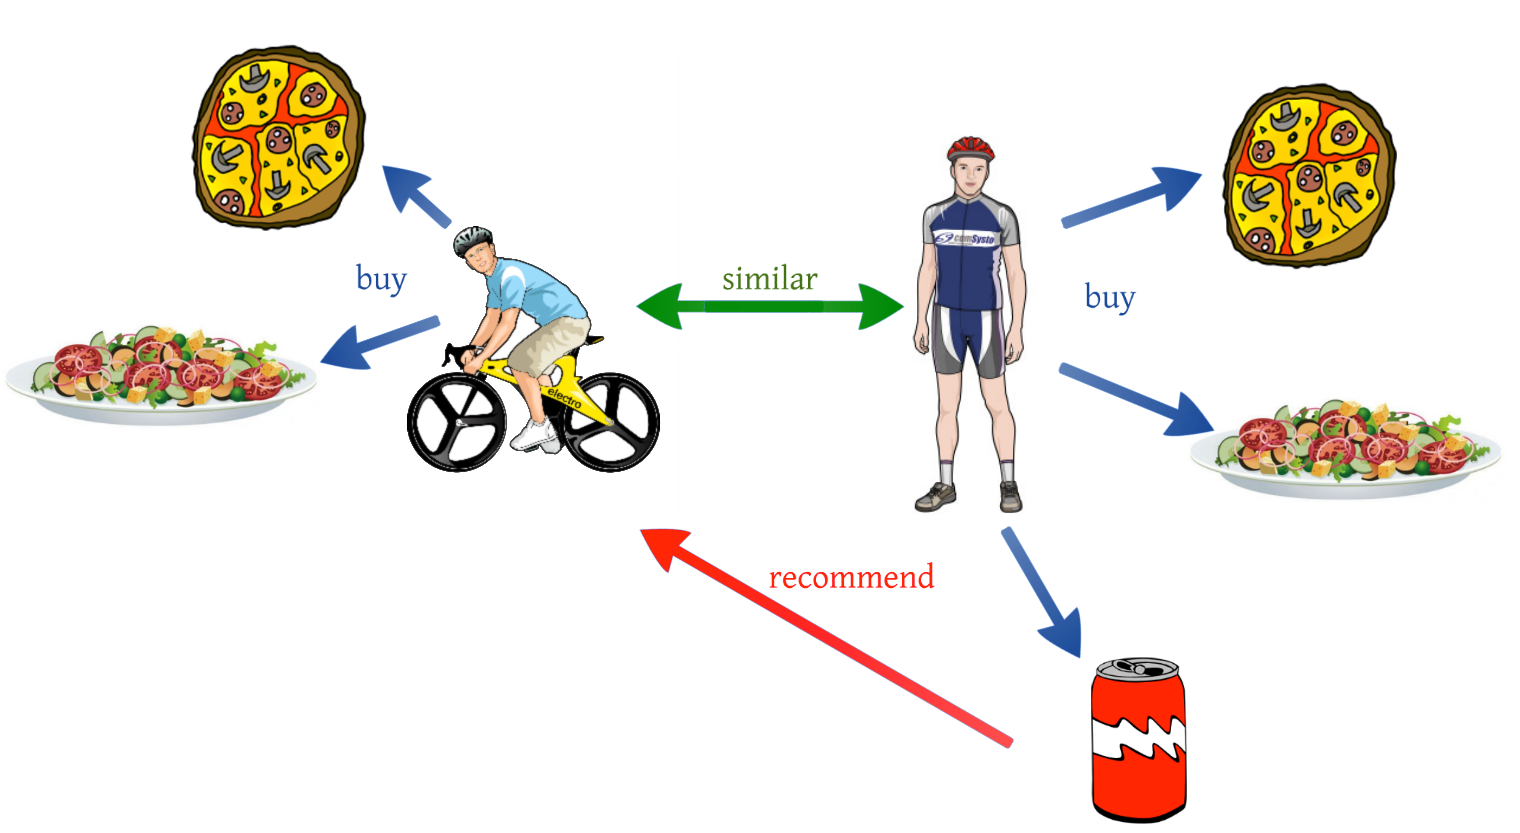
\includegraphics[width=\columnwidth,height=\paperheight,keepaspectratio]{../pictures/collaborative.png}}
	\footnote{Source: \url{https://medium.com/@akhilesh3091999/recommender-system-bb032b16ab67}}
\end{frame}

\begin{frame}{Item-based filtering}  
	\begin{block}{Similar items...}
		\begin{itemize}
			\item<1->If two items is rated similarly by a group of people
			\item<2->...these product might be similar
		\end{itemize}
	\end{block}
		\begin{exampleblock}{Example...}
			\begin{itemize}
			\item If Alex, Sanne and Marthe like skincare product \textit{X} and \textit{Y}, and Denise buys skincare product  \textit{Y},  \textit{X} will be recommended. 
			\end{itemize}
		\end{exampleblock}
\end{frame}

\begin{frame}{User-based filtering}
	\makebox[\linewidth]{
		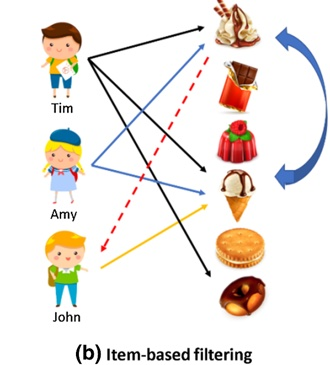
\includegraphics[width=0.5\textwidth]{../pictures/item_based}}
	\footnote{Source: \url{https://predictivehacks.com/item-based-collaborative-filtering-in-python/}}
\end{frame}

\begin{frame}{Example: Amazon}
	\makebox[\linewidth]{
		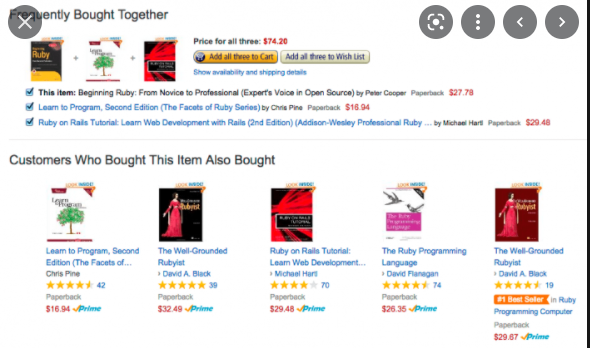
\includegraphics[width=0.5\textwidth]{../pictures/userbased-amazon}}
\end{frame}

%\section[Reflection]{The role of recommender systems in society}

\begin{frame}{Reflection on the role of recommender systems in society}
	\begin{alertblock}{Food for thought}
		\begin{itemize}
			\item <1->Consequences of recommender systems for democratic values in society
		\end{itemize}
	\end{alertblock}
\end{frame}

%\section[Group ass]{Group Assignment}
%\begin{frame}{Build your own recommender system}
%	\begin{alertblock}{Part of the assignment: Build a recommender (20\% of final grade)}
%		\begin{itemize}
%			\item <1->Build a recommender system, based on the insights from this week (week 6). It's up to you to decide whether you build a knowledge-based or content-based recommender system.
%			\item <2->Think about relevant features that you want to use in your algorithm design. Based on which features do you want to recommend content?
%		\end{itemize}
%	\end{alertblock}
%\end{frame}

\begin{frame}{Build your own recommender system}
	\begin{exampleblock}{Practice with the materials!}
		\begin{itemize}
			\item <3-> To be able to do this correctly, it is essential that you understand the code of this week's lab session. 
			\item <4-> Carefully walk through this week's assignment, and to whether questions arise.
			\item <5-> It's up to you to decide whether you want to build a simple knowledge-based or content-based recommender system. Base your selection on the available data columns.
		\end{itemize}
	\end{exampleblock}
\end{frame}

\begin{frame}[standout]
Have fun!
\end{frame}

\begin{frame}[t,allowframebreaks]
	\frametitle{References}
	\printbibliography
\end{frame}

\end{document}